\documentclass[12pt]{article}   	% use "amsart" instead of "article" for AMSLaTeX format
\linespread{1.25}
\usepackage{geometry}                		% See geometry.pdf to learn the layout options. There are lots.
\geometry{letterpaper}                   		% ... or a4paper or a5paper or ... 
%\geometry{landscape}                		% Activate for rotated page geometry
%\usepackage[parfill]{parskip}    		% Activate to begin paragraphs with an empty line rather than an indent
\usepackage{graphicx}				% Use pdf, png, jpg, or eps§ with pdflatex; use eps in DVI mode
								% TeX will automatically convert eps --> pdf in pdflatex		
\usepackage{amssymb}
\usepackage{eurosym}
\usepackage[affil-it]{authblk}
\usepackage[utf8]{inputenc}
\usepackage[english]{babel}
\usepackage{caption}
\captionsetup{font=bf}
 
\setlength{\parindent}{4em}
\setlength{\parskip}{1em}

\usepackage{graphicx} %package to manage images
\graphicspath{ {/home/barrymun/Documents/report-latex/texfiles/} }

\usepackage{tikz}
\usetikzlibrary{matrix,chains,positioning,decorations.pathreplacing,arrows}



\usepackage{listings}
\usepackage{color}

\definecolor{dkgreen}{rgb}{0,0.6,0}
\definecolor{gray}{rgb}{0.5,0.5,0.5}
\definecolor{mauve}{rgb}{0.58,0,0.82}

\usepackage[most]{tcolorbox}

\tcbset{
    frame code={}
    center title,
    left=0pt,
    right=0pt,
    top=0pt,
    bottom=0pt,
    colback=gray!70,
    colframe=white,
    width=\dimexpr\textwidth\relax,
    enlarge left by=0mm,
    boxsep=5pt,
    arc=0pt,outer arc=0pt,
}


\lstset{frame=tb,
  language=Java,
  aboveskip=3mm,
  belowskip=3mm,
  showstringspaces=false,
  columns=flexible,
  basicstyle={\small\ttfamily},
  numbers=none,
  numberstyle=\tiny\color{gray},
  keywordstyle=\color{blue},
  commentstyle=\color{dkgreen},
  stringstyle=\color{mauve},
  breaklines=true,
  breakatwhitespace=true,
  tabsize=3
}

\usepackage{amsmath}
\usepackage{caption}
 
\DeclareCaptionType{mycapequ}[][List of equations]
\captionsetup[mycapequ]{labelformat=empty}

\pagenumbering{gobble}

%SetFonts

%SetFonts


\title{Constructing Complete Paths from Partial Paths in a Directed Graph}
\author{Neil Barry-Murphy}
\affil{Trinity College Dublin}

%\date{}						% Activate to display a given date or no date

\begin{document}

\maketitle

\hfill
\begin{figure}[htp]
\centering{

\includegraphics[scale=0.2]{tcd-logo.jpg}}
\end{figure}

\hfill
\begin{center}
Under supervision of Professor Stephen Barrett
\end{center}
\thispagestyle{empty}

\newpage

\pagenumbering{roman}
\section*{Declaration of Authorship}
I, Neil Barry-Murphy, declare that the following dissertation, except where otherwise stated, is entirely my own work; that it has not previously been submitted as an exercise for a degree, either in Trinity College Dublin, or in any other University; and that the library may lend or copy it or any part thereof on request.

\noindent
Signed:

\noindent
Date:

\newpage

\section*{Acknowledgements}
I wish to express my deepest thanks and appreciation to my supervisor, Professor Barrett, for his ongoing support throughout the year. His wealth of knowledge, information and research assistance proved invaluable to me throughout the course.

\noindent
To my parents, my brother Colin and aunt Ann, without whom my many years of academia would not have been possible, I am forever grateful.

\noindent
I would also like to take the opportunity to thank my friends Aaron, Ian and Evin. Their continuous encouragement, generosity and support was inspirational.

\noindent
Finally, I wish to thank Eva. You revealed to me the light at the end of the tunnel.
\newpage

\section*{Abstract}
Information is one of the most important factors in the determination of the success or failure of any application or system, irrespective of the size of the user base. To paraphrase the philosopher, Sir Francis Bacon; “Information Is Power”. Without information, it is impossible to accurately derive solutions for any problem in any named area of expertise.

Let us imagine, however, that all information required to complete a particular task is available, but we cannot effectively complete the task for whatever reason. For example, queries to a KB take an inordinate amount of time, the data available is poorly or incorrectly formatted or the most useful data is the most difficult to retrieve.

This research project analyses the effectiveness of crowd caching, or smart caching, in order to efficiently retrieve route information from a GDB. The returned route may already exist as a complete path, or may be derived from a series of interconnecting partial paths in the GDB.

Therefore, we must analyse the ability of such a system to improve application performance, reduce costs and adequately display the results of a user query.
\newpage

\section*{Acronyms and Abbreviations}

API
\hspace{13.5mm}
Application Programming Interface

\noindent
ASCII
\hspace{9.5mm}
American Standard Code for Information Interchange

\noindent
CPCS
\hspace{10mm}
Complete Path Construction System

\noindent
GDB
\hspace{11.5mm}
Graph Database

\noindent
JSON
\hspace{10.5mm}
JavaScript Object Notation

\noindent
KB
\hspace{15mm}
Knowledge Base

\noindent
MVC
\hspace{11.5mm}
Model View Controller

\noindent
N4J
\hspace{14mm}
Neo4j

\noindent
P2N
\hspace{13.2mm}
Py2neo

\noindent
SL
\hspace{16.5mm}
Storstockholms Lokaltrafik

\noindent
TFLB
\hspace{10mm}
Trafiklab

\newpage

\tableofcontents
\newpage

\pagenumbering{arabic}
\section{Introduction}
\subsection{Background}
Application or software performance improvements, cost reduction (with a particular emphasis on bandwidth and processing power, discussed in research objectives) and product aesthetics are of paramount importance. Particularly to any individual, company, university or other research body attempting to construct a system that gathers information by some means. User input is one such example, as it will yield a desired result or set of results based on some interpretation or series of computations which focus on a certain segment, or all, of this previously collected knowledge.

All information collected must exist digitally in order that it may be referenced, traversed, modified or deleted. The knowledge base must also allow for new additions. A Directed-Acyclic Graph (DAG) is a complex data structure which can be modelled as a database, i.e., the knowledge base in question. The order in which the nodes are connected is important, as it differentiates between data pertaining to one direction, and its opposite, even though the nodes in both data sets are the same. The connections, or edges to be precise, in these same data sets are very different.
	
There are many computational problems that are solved, or partially resolved, through the application of a DAG to such an issue. Practical examples include compile-time optimizations for list scheduling algorithms using directed-acyclic graphs [7], and the determination of (any) existing links between prices of commodity markets and their respective governing transport markets regarding the provision of the aforementioned goods [14].

\newpage

\subsection{Project Definitions}
\subsubsection{Stop}
A stop is a physical location where a population can board some type of public transport: bus, train or tram. A stop will be represented as a node in the GDB; refer to the design section of this document.

\subsubsection{Connection}
A connection is the intermediate relationship between a current stop, the next stop and the previous stop. Each of these stops are only accessible via each other; a stop cannot be skipped if following the transit guideline for the route containing these stops. Of course, a stop can be a link for multiple different routes, so many connections involving the same stop may exist. A connection will be represented as an edge in the GDB; refer to the design section of this document.

\subsubsection{Leg}
A route is comprised of a single or multiple legs. A leg is broken into two stops, and the connection that exists between them. These two stops are referred to as the origin and destination, but it is important not to confuse this naming convention with the actual origin and destination set by the user. The destination of the previous leg within a route is the origin of the current leg of the same route. The TFLB API (refer to the Literature Review section for more detailed information) returns all data in this format ensuring a simplistic route information to path mapping process.

\subsubsection{Route}
A route is defined as the series of connections between stops in the TFLB open API that forms a complete and unbroken link between an origin and a destination stop that are specified by any user of the CPCS. The stops and connections that form a complete route between the origin and destination are not outlined by the user.

\subsubsection{Path}
Within the CPCS, a path is defined as a collection of two or more nodes connected by edges, or paths within the graph database. A path cannot be generated from the existence of a single node only.

A node represents a stop, and an edge represents a connection between two stops. For example, let us imagine two stops; Stockholm (A) and Arlanda (D). A user of the CPCS wishes to get from A to D, but must go through B and C beforehand. Thus, the path is displayed in Figure 1 hereunder:

\noindent
\begin{figure}[htp]
\centering{
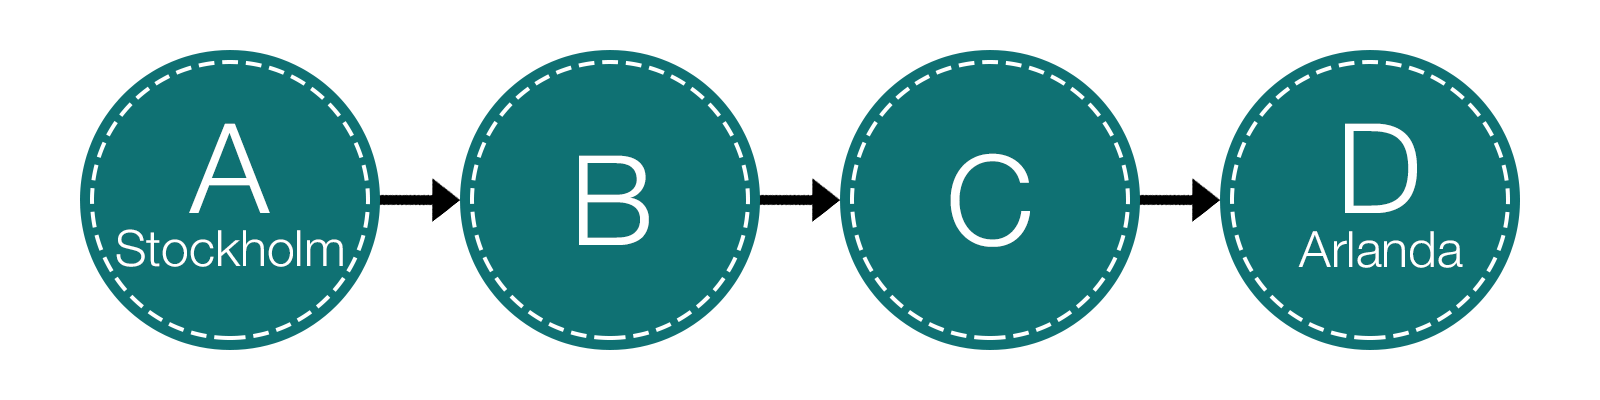
\includegraphics[scale=0.2]{AthroughBCD.png}}

\caption{Sample route from A to D, through B and C.}
\end{figure}

\noindent
This path also represents the shortest possible path between stops (A) and (D) in the graph database.

\newpage

\subsection{Motivation}
Public transportation is a fundamental component to the underlying structure of any country, region or state. As the population of a region continues to rapidly expand, the demand for public transport continues to exponentially increase [1]. There are many software solutions that exist which can efficiently derive some route from A to Z, for example, but these solutions, in general, are not open source. The route is provided free of charge and is returned very quickly. A registration process is not required [13]. However, it is impossible to modify this software for personal use (not open source), and this is an important requirement for the purposes of many companies and/or private individuals. Solutions exist which allow for personal integration with the above software, but they are expensive. In addition, many transport operators (or other companies/individuals) may require complete control of the route finding software in their possession, such as the area or region in question, supported transport types, ticket pricing information and custom result formatting. This is not always achievable when employing third party software.
	
There are many publicly available APIs which provide real-time traffic information for public transport systems. The majority of these transport systems are specific to a region or country, which is a suitable limiting factor for the purposes of this research project.  The API that is used for this particular study is the TFLB open API, which provides route information gathered from many public transport operators within Sweden. Such operators include Storstockholms Lokaltrafik (SL [23]). Registration to TFLB is compulsory so that individual API access keys can be distributed in order to monitor usage statistics for all members. Service fees vary from API to API (there are many, and the exact API names are outlined in the Literature Review section). The threshold is high for an individual, but not for a larger company making several thousand API calls per day. Thus, the target market of this research project are companies (potentially public) or private firms with an extensive user base. TFLB provides usage documentation, but a web application is required to manage three core issues pertaining to this study which are outlined in the following paragraphs. All query results from TFLB are returned in JSON format.
	
Therefore, the pivotal motivating factor behind this research project is the combination of an intuitive frontend display and navigation system with a large-scale route derivation system which takes advantage of all route data supplied by the open API TFLB. Essentially, third party route derivation software cannot be used to complete this objective. Furthermore, the final product must address three fundamental issues; responsiveness, cost reduction and intelligible, aesthetic route presentation for the user.
	
The first issue, responsiveness, this means that a noticeable performance improvement must be perceived by the end user. When a previously cached route is requested, and all legs of the route are valid, the rate at which the result is returned must be significant. The same suggested performance improvement can be applied to the derivation of a complete path from a partial path; the route does exist in the GDB, but was not a route which was directly requested from TFLB and stored in the database.
	
Substantial expenses are associated with all large companies. The reduction of these costs is of the utmost importance to the success of the business. TFLB allows for a maximum number of calls to an API, after which a charge is incurred per request. This charge varies from API to API. The proposed application will eliminate the need for a request to TFLB if the route directly exists, or if the route can be constructed from a series of partial paths. In theory, costs will be greatly reduced for large scale systems with a sizable user base (refer to the Results and Conclusions section for more information on testing procedures), as a query to the GDB is not regarded as an expense, unlike a query to the TFLB API. In contrast, however, the performance of smaller systems that do not regularly request the same route (while it remains valid) will actually decline, as the time to request a single graph route lookup and a TFLB inquiry is clearly greater than the time to make a request to TFLB in isolation. This is the amortized cost of the transaction.

The third and final major addressable issue, the presentation of all results retrieved must appear aesthetic. It is very difficult for a user to interpret a JSON dataset, thus the route must be laid out clearly, with an emphasis placed on highlighting the necessary stops, connections and departure and arrival times. Google Maps [13] displays the result of a route query in an effective manner, and the objective for this particular task is to closely replicate this structure.

\noindent
\begin{figure}[htp]
\centering{
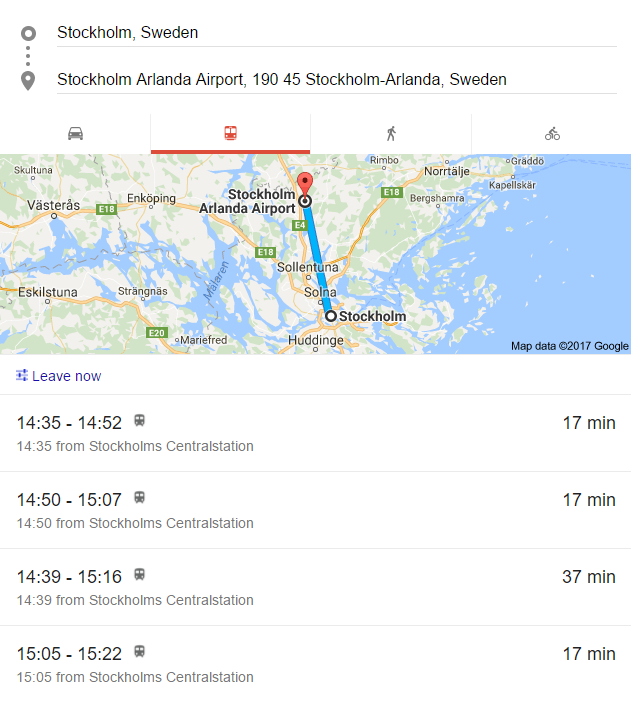
\includegraphics[scale=0.5]{sto-to-arl.PNG}}

\caption{Screenshot of Google route data; Stockholm to Arlanda.}
\end{figure}

A search refers to the derivation of some route from the input parameters set by the user. These include some origin and destination location. Thus, it is evident that a complete system is required to effectively manage the three dominant issues outlined above; a web application. The construction of this feature associated with the overall project is summarized in the Design section of this report.
	
A further motivational aspect is the lack of publicly available software that adequately addresses the above issues, while permitting a system administrator or developer to completely govern all aspects of the software. The API route data module selection (TFLB may not prove suitable in all use cases), a user registration feature (monitor individual requests in greater detail for a more in-depth analysis), modes of public transportation selection (for example, only providing routes specific to trains) and modification of the aesthetics of the CPCS web application (for a more personalized style) must be permissible to any other potential user of the CPCS.
	
A personal interest in graph theory has also proved influential to the selection of this research topic. It is acutely applicable to the route retrieval problem, as it is possible to visualize graph nodes as route stops and graph edges as route connections. This is where the parameters of the edges contain specific details for each leg of the journey, and provide route validation methods.
	
Furthermore, why should data that already exists (in segments) in some form be repeatedly requested? There are only a finite number of stops within a public transportation system and many users (within a large scale system) request similar routes within a short time period. The method employed by Google to quickly retrieve repeated requests is Bigtable [6]. Bigtable is essentially a distributed, multi-dimensional sorted map, thus the inspiration to create a crowd cache (smart caching, refer to Research Objectives paragraph) GDB solution was conceived. The segments referenced above represent the partial path in the GDB. It is entirely possible to convert these partial paths to complete paths. The inference that can be drawn from this is the reduction of costs, the time-saving possibilities (specific details of cost reduction is summarised in Research Objectives), and the opportunity to present data aesthetically for large scale systems that require a publicly available and customisable software solution.

\newpage

\subsection{Research Objectives}
The overall objective was to allow for the construction of a complete path from a series of previously specifically requested pre-existing paths (a new query that can be satisfied without the use of the TFLB API). All of these complete paths within the GDB become partial paths in order to satisfy this new query to ensure that a complete path is produced. All objectives of this investigation are outlined as follows:

\begin{itemize}
	\item Construct a user interface whereby it is possible for an individual to search for a route (defined above). The user must be able to specify the origin and destination of this route.
	\item Create a backend system that will remotely query the open API TFLB (refer to Literature Review section for more information) so that the parameters of the search (the origin and destination) are used to retrieve any route details.
	\item The returned results will contain many routes, and that is assuming that the route remains valid within the TFLB API. The shortest route must be prioritised using Dijkstra’s Algorithm, with respect to the arrival and departure times. This route is then returned to the user.
	\item Physical distances between stops in any route are calculated using the Haversine Formula. This formula computes the straight line geographical distance between two sets of latitude and longitude coordinates. These are supplied by the TFLB API.
	\item Each shortest route will be added to the GDB. Nodes will represent the stops and edges will represent the connection that exists between two stops, in the event of the existence of such a connection. This includes routes that have been directly queried from TFLB, and now exist in the GDB (complete paths), or routes that exist in the database only as a result of the compilation of many other previously queried routes (partial paths). Partial paths are paths that have not been queried from the TFLB API.
	\item Dijkstra’s Algorithm is also used to compute the shortest route when querying directly from the GDB when a call to TFLB is not required.
	\item The graph must always be queried for a route before the TFLB API, otherwise the potential time and monetary savings will never be realised. The only exception to this rule occurs when the GDB does not contain any elements (nodes or edges).
	\item Suggested performance improvements achieved through TFLB API hit reduction. Query time differences (if any) which highlight the effect of this feature implementation are presented in the Results and Conclusions section of this report.
	\item The primary features of cost reduction, with respect to the title of this document are bandwidth and processing power. The “cost” keyword is essentially a filter for these attributes.
	\item Results generated from the user's original query (the desired route) returned either from the GDB or TFLB must be presented to the user in an aesthetic manner in order that they are comprehensible.
	\item In summary, the main objective is to answer route questions pertaining to crowd-sourcing, where crowd-sourcing is the combination of many results (route queries) and to derive some new route which may not exist directly within the GDB.
\end{itemize}

The system developed to display the results of these findings will be called the “Complete Path Construction System”, or CPCS succinctly. The CPCS is designed to reduce lookup times for routes, for routes within routes, or routes that can be constructed from the pre-existence of other routes connected by paths that already exist in a database.

\newpage

\subsection{Challenges}
A series of challenges were encountered during the design, construction, testing and analysis phases of this research project, and are outlined below:

\begin{itemize}
	\item If a route does not exist, or the parameters of the search (the origin and destination locations) are invalid, then the CPCS must correctly handle the error and appropriately notify the user.
	\item The connection (edge) between each stop (node) in the GDB must be validated whenever they are involved in a query relating to the GDB. For example, an edge with an associated departureTime parameter that stores a timestamp value lower than that of the current time of the system is invalid. Dates that have expired are also considered invalid.
	\item The Haversine Formula, which is used to calculate the geographical distance between two points cannot be used as the determining factor of a connection, or of a complete route when taking into consideration the definite shortest path. It is rarely, if ever, possible to travel from one stop to another in a straight line. This is merely used as a check to eliminate much longer routes, where distances vary by several kilometres. For all other instances, the shortest route must be determined by total travel time and arrival time through the application of Dijkstra’s Algorithm. This means that the relevancy of edge weight when applying Dijkstra’s Algorithm using the distance between the nodes as the metric of computation is completely removed. This methodology will be further elucidated in the Literature Review section of this report.
	\item Edges that connect two nodes must be directional, thus producing the desired directed GDB. Only the edges are altered when updating the graph, as node information remains static, i.e., a stop name will not change suddenly. Two connections can exist between two nodes, and the direction of these connections can be completely opposite. Bidirectional edges cannot exist.
	\item There are over thirty possible decisions that can be considered by the CPCS with respect to the extraction of a final route based on the input parameters of the user. These rules govern the methods in which the data can be retrieved: i) through the use of the GDB if the route exists as a complete path, ii) or can be derived as a partial path from a series of complete paths, iii) or by querying directly from the TFLB API. All possible decisions are outlined in the Design section of this report.
	\item Multiple nodes can exist harmoniously in the GDB, even if they are assigned the same siteId. However, the stopId parameter of each node must be unique. The siteId (integer) refers to the general location of the stop such as Arlanda, Marsta, Stockholm. The stopId (integer) defines the transport method type, such as the bus, train, tram or boat, at that particular location for a given time (the departureTime of the origin node in the current leg of the route). The system must allow for multiple nodes that have been assigned the same siteId.
	\item Upon retrieval of a partial path (a route that has not been directly queried from some previous search), each leg of the journey must be validated. Only the first leg of a journey must be validated when new routes are inserted into the GDB.
	\item Due to the nature of the data (all information retrieved is presented in Swedish), ASCII characters must be stripped from the data before it can be inserted into the GDB. The prevents certain Python [20] TypeError issues, which are explained in more detail in the Design section of this report.
	\item The CPCS must display all data aesthetically to the user, but it also must exist as a fully functional tool. A web application was constructed to accompany this design prerequisite in order that this desired functionality was supported. Route insertion and path retrieval features are then integrated efficiently with the CPCS.
\end{itemize}

\newpage

\subsection{Overview of Technical Approach}
An application must be designed to address three core issues of route planning; improved performance (diminished query times), overall reduced system costs (for a large scale user base) and aesthetic result presentation, solved by the construction of complete paths from partial paths using a directed graph.

An account must be created with TFLB in order to request route data. A GDB must be selected to store all routes as complete paths. It is imperative that the direction of the edges in the GDB are directional. An edge relationship cannot exist as a bidirectional link.

Dijkstra’s Algorithm is used to find the shortest path between two parameter nodes in the GDB, the origin and the destination. It is also used to determine the shortest path in a series of routes returned by TFLB.

The web application will return all results in an aesthetic manner, with an emphasis placed on the arrival and departure times of the route. These metrics are an essential part of the calculation of the shortest path with respect to the application of Dijkstra’s Algorithm.

The time taken to derive the shortest route from a series of complete or partial paths in the GDB is recorded and displayed on the resulting web page in order to serve as testing and comparative guidelines. The amortised time of a route calculation is recorded, so the advantages gained or lost when comparing a large and small scale user base can be recorded. However, this improved performance gain for a large scale user base can only be suggested, as a complete test on such a system did not fall within the scope of this research project.

\newpage

\subsection{Report Structure}
Chapter Two, Literature Review, presents a discussion and analysis of the background research which was required to address all issues associated with this project, including an explanation of the factors which influenced all research initiated and completed.

Chapter Three, Methods and Design, transforms the reference material into usable data and system engineering requirements, producing a more formal design description of the overall topic.

In Chapter Four, Implementation, the design is transformed into a concrete implementation. Also discussed are the challenges encountered during the implementation process, and the way in which they were dealt with and ultimately surmounted.

In Chapter Five, Results and Conclusions, an evaluation of the reference material is presented, and to ensure that the results are transparent, the application of this acquired knowledge is included. Any derivations from these results are highlighted, and a section outlining any potential future work is presented.

In Chapter Six, Bibliography, all project references are listed.

\newpage

\section{Literature Review}
This section provides an overview of how the problem of the construction of complete paths from partial paths in a directed graph is managed. The issue is separated into two dominant sections: i) the construction of complete paths from partial paths and ii) directed graphs. An outline of previous work regarding the approach to the construction of complete paths from partial paths, the composition of a GDB and the organization and formal structuring of a directed graph system is provided where necessary.

All analysis regarding the functionality of any complete paths that are constructed, including all testing related to these aforementioned constructed paths, is completed using the real time public transport route information system TFLB. This document attempts to answer these questions, and reveal the solutions to these issues (if any) by compiling previous research and applying classifiers to online data.

\subsection{Construction of Complete Paths}
\subsubsection{Introduction to Graph Theory}
In order to understand the concept of a path we must understand the notion of a graph. “Introduction to Graph Theory” [30] accurately defines a graph as a structure that can be summarized with the formula:

\hfill
\noindent
\[ G = (N,E) \]

\noindent
which states that a graph is composed of a set of nodes ‘N’, and a set of edges ‘E’. Nodes may or may not be connected by these edges, and may link to any other node in the graph, but nodes cannot be linked to other nodes without an edge. A connection between two nodes within the CPCS is an edge, but includes a series of parameters, or attributes, and these are associated with all individual edges. These parameters include distance, departureTime and departureDate. All edges are assigned an id parameter by the N4J [18] GDB (defined in the implementation section) upon creation. This value cannot be modified, but an edge associated with an id parameter may be deleted.

\subsubsection{Mapping Stops and Connections}
There are three fundamental reasons which clarify the selection of a graph to represent the CPCS database; flexible graph modelling constructs, improved performance of a GDB versus a relational database and the ability to apply Dijkstra’s algorithm to acquire the shortest path between two nodes in the GDB.

Flexible graph modelling constructs are outlined in the article provided by [22], highlighting that graphs can be viewed as an index that relate nodes to other nodes in the same graph by edges (stop connections) when relationships between objects in the graph are considered node partitions. This means that when a specific segment of information is requested from the graph, a global analysis of data within the graph is not required, as only the partitions where the relevant data exists is actually queried. This means that graphs are considered a highly efficient data storage and retrieval structure.

In addition, the performance of a graph when querying structural types, modelled as a database, is superior to that of a traditional relational database according to [29]. Performance is key to the success of the CPCS, as the time taken to return a path (assuming that the path, or some series of existing node connections that complete a path) to a user must remain significantly lower when compared with the time taken to query the TFLB open API.

Finally, the application of Dijkstra’s Algorithm to the GDB in order that the shortest path between two nodes can be found, assuming that one or more paths between these nodes exist. The distance parameter for each edge is critical to the success of this calculation, as Dijkstra’s Algorithm computes the shortest path based on the distance, or length, of all edges involved in the calculation, based on [4]. The distance metric is defined in kilometres (km), and demonstrates the importance of this measurement.

\subsubsection{Path definition with respect to the CPCS}
A path, within some graph ‘G’, is defined as the finite, non-empty sequence:

\hfill
\noindent
\[ P = \sum n0, e1n1, e2n2 … eknk \]

\noindent
where ‘n’ represents a node and ‘e’ represents an edge in the same graph ‘G’. This states that ‘P’ here is the path from the origin node ‘n0’ to the destination node ‘nk’, where ‘e1’ through ‘ek’ represents the connection between each corresponding node in path ‘P’, according to [2].

In the Introduction section a route was defined as the series of connections between stops that form a complete and unbroken link between an origin and a destination stop (Introduction). If some route exists in a GDB, then the CPCS considers that route to be a path (Introduction provides a definitive example), assuming that the path adheres to the rules outlined by the above definition.

\newpage

\subsubsection{The purpose of complete and partial Paths}
Without the existence of a path (or paths) within the GDB, we cannot construct a complete path from a pre-existing partial path or set of partial paths, as the path does not exist.

Furthermore, if a path does not exist, then the application of Dijkstra’s Algorithm to the CPCS GDB is counterproductive, as the shortest path cannot be derived if no path exists. This significantly reduces the CPCS performance time, as a query is made to extract the shortest time, which will not yield a result, and this means that a request to the TFLB API is required, thus increasing the overall response time of the CPCS for this particular instance.

\subsubsection{Dijkstra’s Algorithm}
Dijkstra’s Algorithm is an algorithm used to find the shortest path between all nodes in a graph, GDB or some other graph structure, or the shortest path only between two given nodes in the same graph [8].

The application of Dijkstra’s Algorithm within the CPCS GDB, given an origin and destination node (only two input nodes are required) will return the shortest path, assuming that these two nodes are linked by a series of edges and other interconnecting nodes. If no such connection exists, then Dijkstra’s Algorithm cannot be applied.

\subsubsection{How does Dijkstra’s Algorithm work?}
According to (Ahuja, 1988), the most effective approach regarding the implementation of Dijkstra’s Algorithm involves the use of a heap to manage calculations. A heap is a tree-based data structure that must satisfy the “heap property”; if node ‘X’ is the parent of node ‘Y’, then the value of the node ‘X’ is ordered with respect to the value of the node ‘Y. This order is continuously applied to the lower levels of the heap structure alongside the execution of a coded implementation of Dijkstra’s Algorithm.

\noindent
\hfill
\begin{figure}[htp]
\centering{
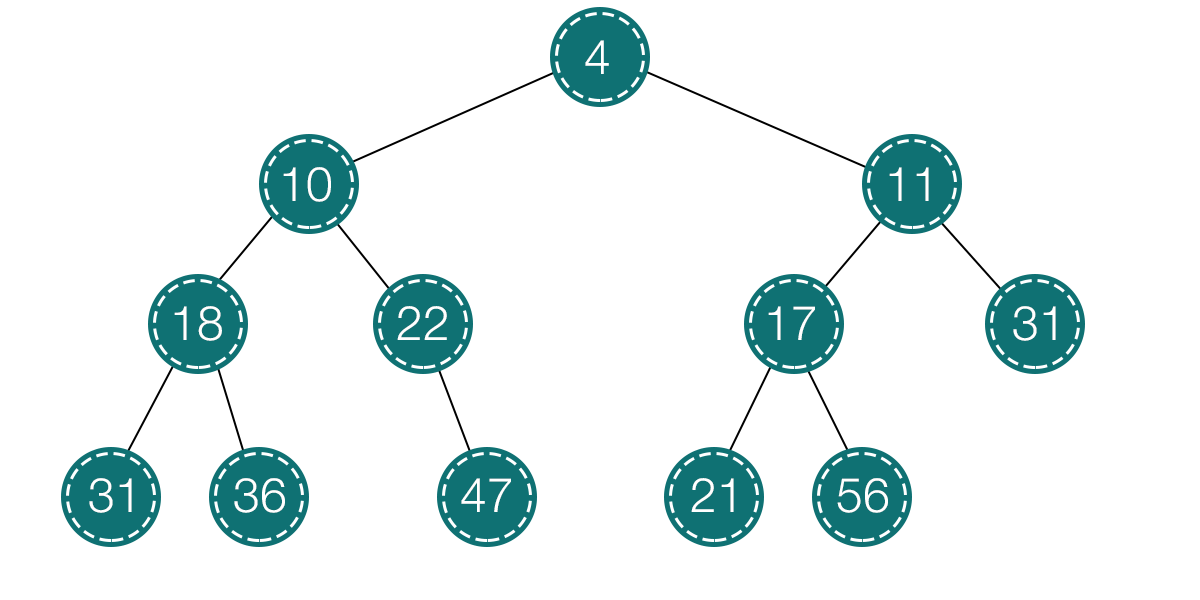
\includegraphics[scale=0.3]{heap.png}}

\caption{Sample Heap.}
\end{figure}
\hfill

There are two graph problems addressed through the use of Dijkstra’s Algorithm. In the instance that at least one path exists between any two nodes in a given graph ‘G’, then it is possible to find the shortest path between between all ‘N’ nodes in ‘G’, or the shortest path between two given nodes, ‘P’ and ‘Q’ only (Dijkstra, 1959). For the purposes of the CPCS, only the second solution to the shortest path problem will be applied, as the only desired result is the shortest path between an origin and a destination node.

\noindent
The second problem relates to finding the shortest path between all nodes in a graph. This problem is explained in the following guidelines.

\noindent
Step 0: Set an initial (origin) node and a destination node in the graph. These nodes must exist.

\noindent
Step 1: Assign to every node a distance value. The distance of the initial node must be set to zero, and the distance of all other nodes in the graph must be set to infinity. Dijkstra’s Algorithm will retrieve the temporary distance assigned to the relationship between a node and another linked node by default, and will attempt to improve these values with every iteration.

\noindent
Step 2: Set the initial node as the current node. The current node is marked as a “visited” node. All other nodes are marked as “unvisited”, until they become the focus of the calculation (the current node). All “unvisited” nodes in the graph are contained within a named list.

\noindent
Step 3: Focus on the current node. Let us assume that the current node is not the initial node (node ‘A’), and node ‘A’ has been marked as “visited”. Compute the distances between the current node (node ‘B’) and all neighbor nodes. A neighbor node is a node that can be linked by a single edge to the current node. Let us assume that the distance from initial node ‘A’ to current node ‘B’ is 8. Compare the newly calculated distance between the current node ‘B’ and a neighbor node ‘C’. If this new value is less than the previously assigned temporary distance, set the distance as the newly calculated value (the distance between the current node and a neighbor node). Let us assume that the distance from the current node ‘B’ and the neighbor node ‘C’ is 3. If the newly calculated distance plus the distance value already assigned to the current node (the distance from node ‘A’ to node ‘C’, through node ‘B’; 8 + 3 = 11) is less than the distance already assigned to this path (should a distance value from node ‘A’ to node ‘C’, through node ‘B’ exist), then set this distance as 11. Otherwise, do not alter this value.

\noindent
Step 4: When all neighboring nodes, including the current node ‘B’, have undergone the calculations outlined in step 3, the current node is marked as “visited”, and removed from the “unvisited” list. If a node does not exist in the “unvisited” list, then it will not be re-checked by the algorithm.

\noindent
Step 5: If the destination node has been marked as “visited”, or if no connection exists between the origin node and the destination node, then we terminate the program and the algorithm is complete. Otherwise, repeat step 3.
	Assuming that the shortest path, or a single path (which is considered the shortest path) exists between the origin and the destination nodes, this path (the result) is returned to the CPCS.

\subsubsection{The Cypher Query Language}
Dijkstra’s Algorithm, represented using the native Cypher Query Language function:

\hfill
\noindent
\[shortestPath( (from) - [:relationship] -\textgreater (to) ) \]
\hfill

This is used to calculate the shortest possible path between an origin node and a destination node within a GDB, assuming that both nodes, and some relationship or series of relationships (which may include other interconnecting nodes) between them actually exists.

It is imperative to employ the “shortestPath” function native to the Cypher Query Language, as this allows for the computation of the shortest path between two specified nodes without the additional complexities of considering the weight of each individual edge during the calculation [15].

\newpage

\subsubsection{Dijkstra's Algorithm and the Cypher Query Language}
The application of Dijkstra’s Algorithm to the CPCS is not only a matter of converting the algorithm specifications into a programmable representation, but also involves the use of the Cypher Query Language to query the N4J GDB for the shortest path between an origin and destination node, should such a path exist in the database. This topic also relates to the previous discussion regarding the definition of a path; a path existing as the portrayal of some route in the GDB.

Cypher is a declarative, SQL-based query language used to visually describe graph patterns by means of ASCII-art syntax. It allows a user to determine the desired database actions: i) insert, ii) update or iii) delete items from the GDB without specifying the exact procedure. In conjunction with this information, the Cypher graph Query Language is equipped with a dedicated function that returns the shortest path between two nodes without taking into consideration edge weights [15]. Edge weights represent the distances between two nodes that are directly linked in the database. This action considerably improves the performance of the CPCS.

\newpage

\subsection{Directed Graphs}
\subsubsection{Definition of a Directed Graph}
In graph theory, a directed graph is a set of nodes and edges that are connected together, where all edges are directed from one node to another. The direction of the relationship between two nodes can be forward facing or backward facing. Multiple relationships can even exist between the same two nodes. A directed graph can also be referred to as a directed network.

The direction of a relationship must be specified upon creation of that relationship, before it can be assigned as a correct functional link between two nodes in the CPCS graph [5], assuming that ‘G’ is a directed graph where the set of nodes (or vertices) are defined as:

\hfill
\noindent
\[N = {1, 2, ..., k} \]
\hfill

\noindent
where k is the total number of nodes in graph ‘G’, and the edge set is constructed as:

\hfill
\noindent
\[E \subseteq N \times N \]
\hfill

\noindent
under the provision that each edge is assigned a directional reference.

\newpage

\subsubsection{Trafiklab (TFLB)}
Trafiklab [24] is an open API that allows users to easily request route information when given a set of input parameters including the origin and destination points of the journey set by the user. Route, Stop and other requested data is returned in JSON format, and is accessed and manipulated on the client side of the system. TFLB is used to collect this information as it is an open API, meaning that all system data is publically available for personal and commercial intentions. This information is the primary source of the N4J graph data. Nodes in the graph represent stops in the route, while edges represent the connections (relationship) between each stop.

The graph will systematically map all connections between all relevant stops in a query based on the input data from TFLB, and return results to the user of the system. If the same route, or a subset of the route is requested within a certain time period (defined in the Design section), the data will be requested from the graph, and not TFLB, theoretically resulting in faster results returned to the user following a search query. A query, in this instance, is defined as the request for route information between a predetermined origin location and destination set by the user.

\subsubsection{Directed Graphs and the CPCS}
The path definition includes the existence of a route in the CPCS GDB, and that route is subsequently considered a path. A path can exist as an origin and a destination only, with some specified edge connecting both of these nodes. It can also exist as an origin, a destination, a series of nodes between the former and all edges representing connections between each node in the path.

Focus is now centred on the connections between all nodes in a given path (the edges). It is of paramount importance that the connection between each node is directed in some manner, either forwards or backwards. It is also important to acknowledge that multiple connections can exist between the same two nodes in the CPCS GDB. Consider the following example; a user searches for a route using the CPCS, and sets the origin and destination locations as Stockholm and Arlanda respectively. Let us assume that this route involves travel between four stops, by train, including both locations set by the user. We may also assume that this route already exists in the GDB. The route is mapped as follows:

\noindent
\hfill
\begin{figure}[htp]
\centering{
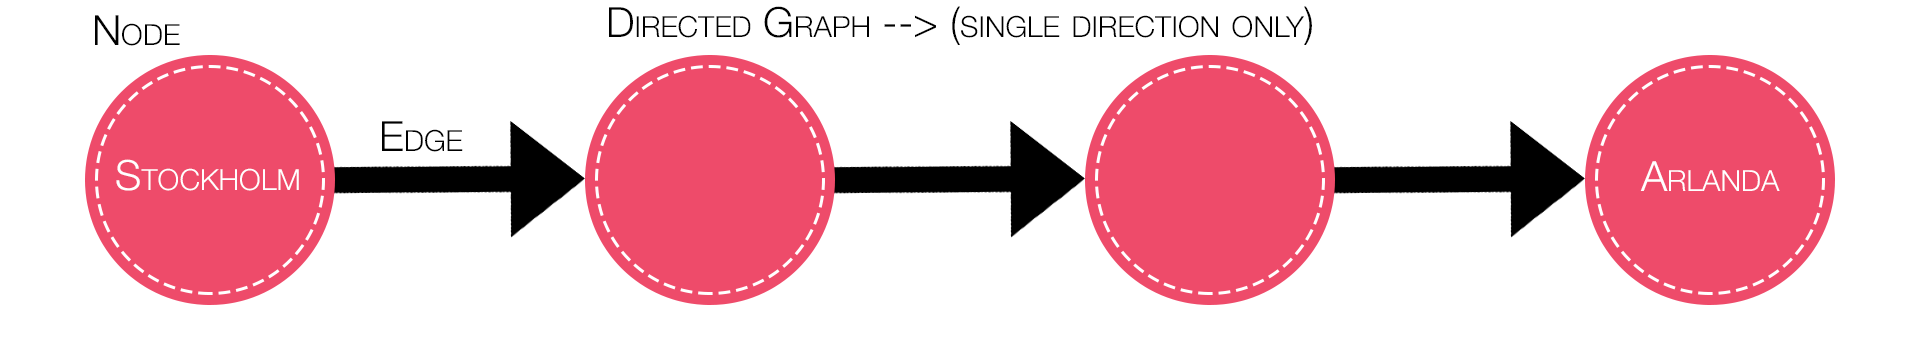
\includegraphics[scale=0.2]{directed-graph.png}}

\caption{Sample Route Data mapped within the GDB.}
\end{figure}
\hfill

\noindent
The path is initialized at node ‘A’ (the route begins at stop ‘A’). The next node in the path is node ‘B’. All route information is requested from the TFLB open API, and parsed by the CPCS so that the route is stored in the GDB (more information is provided on this topic in the Design section of this document). Route information regarding the connection between stops ‘A’ and ‘B’ is also provided by TFLB. The same is true for the connection between stops ‘B’ and ‘C’, stops ‘C’ and ‘D’ and stops ‘D’ and ‘E’. The information provided is used to map out the parameters associated with each edge: distance, departureTime, departureDate and id (default). The direction of this edge is automatically set by the GDB, as the nature of the relationship is defined by the origin and destination of all legs in the route. In the above example, the route contains three legs returned within a single list:

\newpage

\noindent
\hfill
\begin{figure}[htp]
\centering{
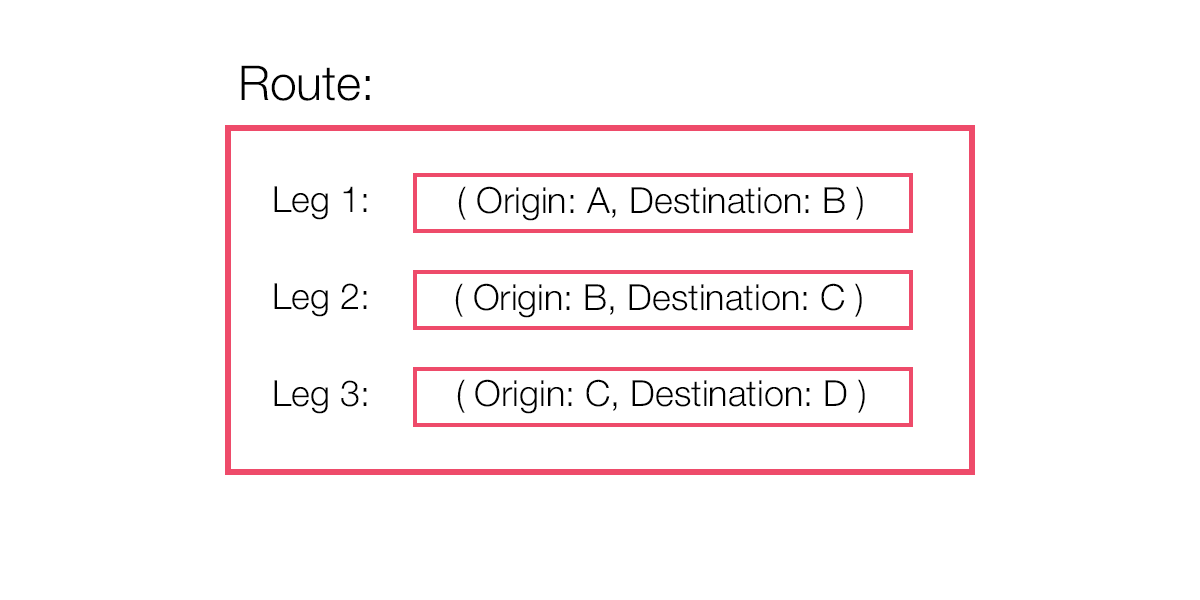
\includegraphics[scale=0.3]{list-with-legs-samples.png}}

\caption{Legs of a route, visualised within a list structure.}
\end{figure}
\hfill

\noindent
Therefore, it is evident that the direction of the relationship is clearly identifiable, and can be set within the GDB in accordance with the manner in which the data is returned from TFLB.

If the relationship between the nodes existed as a bidirectional edge then the graph would be considered an undirected graph and would not be suitable for use alongside the CPCS, as a link between two stops would be regarded as the same connection irrespective of the direction of traversal upon determination of a route. This means that a route from Stockholm to Arlanda would be considered the same as a route from Arlanda to Stockholm, which is completely incorrect. It is impossible for one bus to leave two completely different stations at the same time, on the same date, providing a service for two completely different routes.

\newpage

\subsubsection{Neo4j Trafiklab Route Mapping}
A specific GDB was selected to visually map inbound TFLB route information as complete paths in an attempt to achieve improved performance metrics via faster retrieval times.

N4J is the chosen GDP, and P2N [21] is the designed driver for the Python language, which is used natively by the CPCS (refer to the Implementation section of this document for more information). There are several reasons to support the N4J GDB selection: i) N4J GDB is fully ACID compliant, ii) both full and incremental backups are supported, support for Cypher QL traversal (important for edge weight dependency removal - defined above) and finally iii) N4J is highly optimized for linked data [17].

Thus, based upon the above features supported by N4J, it was determined that this GDB was the most suitable storage method for all inbound requested TFLB route information. Multiple N4J traversal options are also available by using Cypher Query Language to span the GDB when populated.

\newpage

\hfill
\begin{figure}[htp]
\centering{
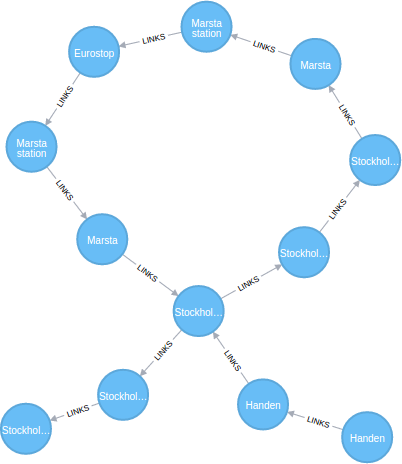
\includegraphics[scale=0.7]{graph-rework.png}}

\hfill
\caption{Screenshot of two overlapping directed routes, taken from Neo4j.}
\end{figure}

\newpage

\subsubsection{The Haversine Formula}
We are now aware that the distance between two nodes in the N4J GDB must be calculated, and included as an edge parameter between the two respective nodes, in order that the application of Dijkstra’s algorithm to the shortest path problem is effective. This distance is calculated by applying the Haversine formula to the latitude and longitude coordinates of the user defined origin and destination locations. This is the most effective method to calculate straight-line point coordinate distances between two locations on the surface of the earth [10]. Unfortunately, the straight-line calculation between two points is not an accurate method to calculate the actual distance between two stops in a given route, as rarely, if ever, are two locations accessible via travelling in a straight line. However, no distance calculation can be retrieved from the TFLB open API, and this method will suffice as a rough estimate of the distance between two points, for the purposes of the shortest path graph traversal computations.

\newpage

\section{Methods and Design}
\subsection{Background Information}
All tools, algorithms and formulas used in the construction of this system are defined in the Implementation section of this document. Refer to the Literature Review chapter for more information. An important factor was the determination of the appropriate TFLB open APIs. The three APIs chosen are SL Stops and Lines 2, SL Location Lookup and SL Travel Planner 2.

\subsection{Route Data, Directed Graph Insertion Mapping}
Stops (nodes) exist in the database, and are distinguished by two main parameters: the stopId and the siteId. A stopId is assigned to a Stop node once a “Travel Planner” API request, which includes this Stop, has been made to TFLB. This stopId is a nine-digit number (in the majority of cases), and is used as a method to quickly find links or relationships (edges) between this particular Stop and other Stop nodes in the database, should they exist.

Similarly, a siteId is also assigned to a Stop node once a Travel Planner API request, which includes this Stop, has been made to TFLB. The siteId is used to determine if a given Stop node actually exists in the database.

All stopId assignations are unique. No two stops can share the same stopId identifier. However, it is possible and not unusual to encounter multiple stops which share the same siteId. This occurs due to the manner in which siteIds are assigned by SL and TFLB. A siteId is determined based on an actual physical location or area. For example, there are many different stop types within the area of Stockholm Central station, and such examples include the bus and train. These stops are assigned the same siteId, as they are all located within the same area or region (all of which are typically within walking distance of each other), but cannot be assigned the same stopId identifier within the SL system, otherwise it would not be possible to distinguish these stops which cater for different transport methods.

Therefore, it can be concluded that using a siteId to check for the existence of relationships (edges) between Stop nodes is considered a safe design feature. Stop nodes that are unlinked in the GDB will force a Travel Planner API request, in the event a request for such a journey is specified by a user.

\noindent
\subsection{Design Phase by Section Analysis}
\noindent

\noindent
The following paragraphs discuss each of the necessary actions that must be performed by the system when dealing with the many requirements of differing search specifications. An architectural diagram is provided below, and each section will refer to some stated segment or mapping outlined in the following blueprint.

\begin{figure}[htp]
\centering{
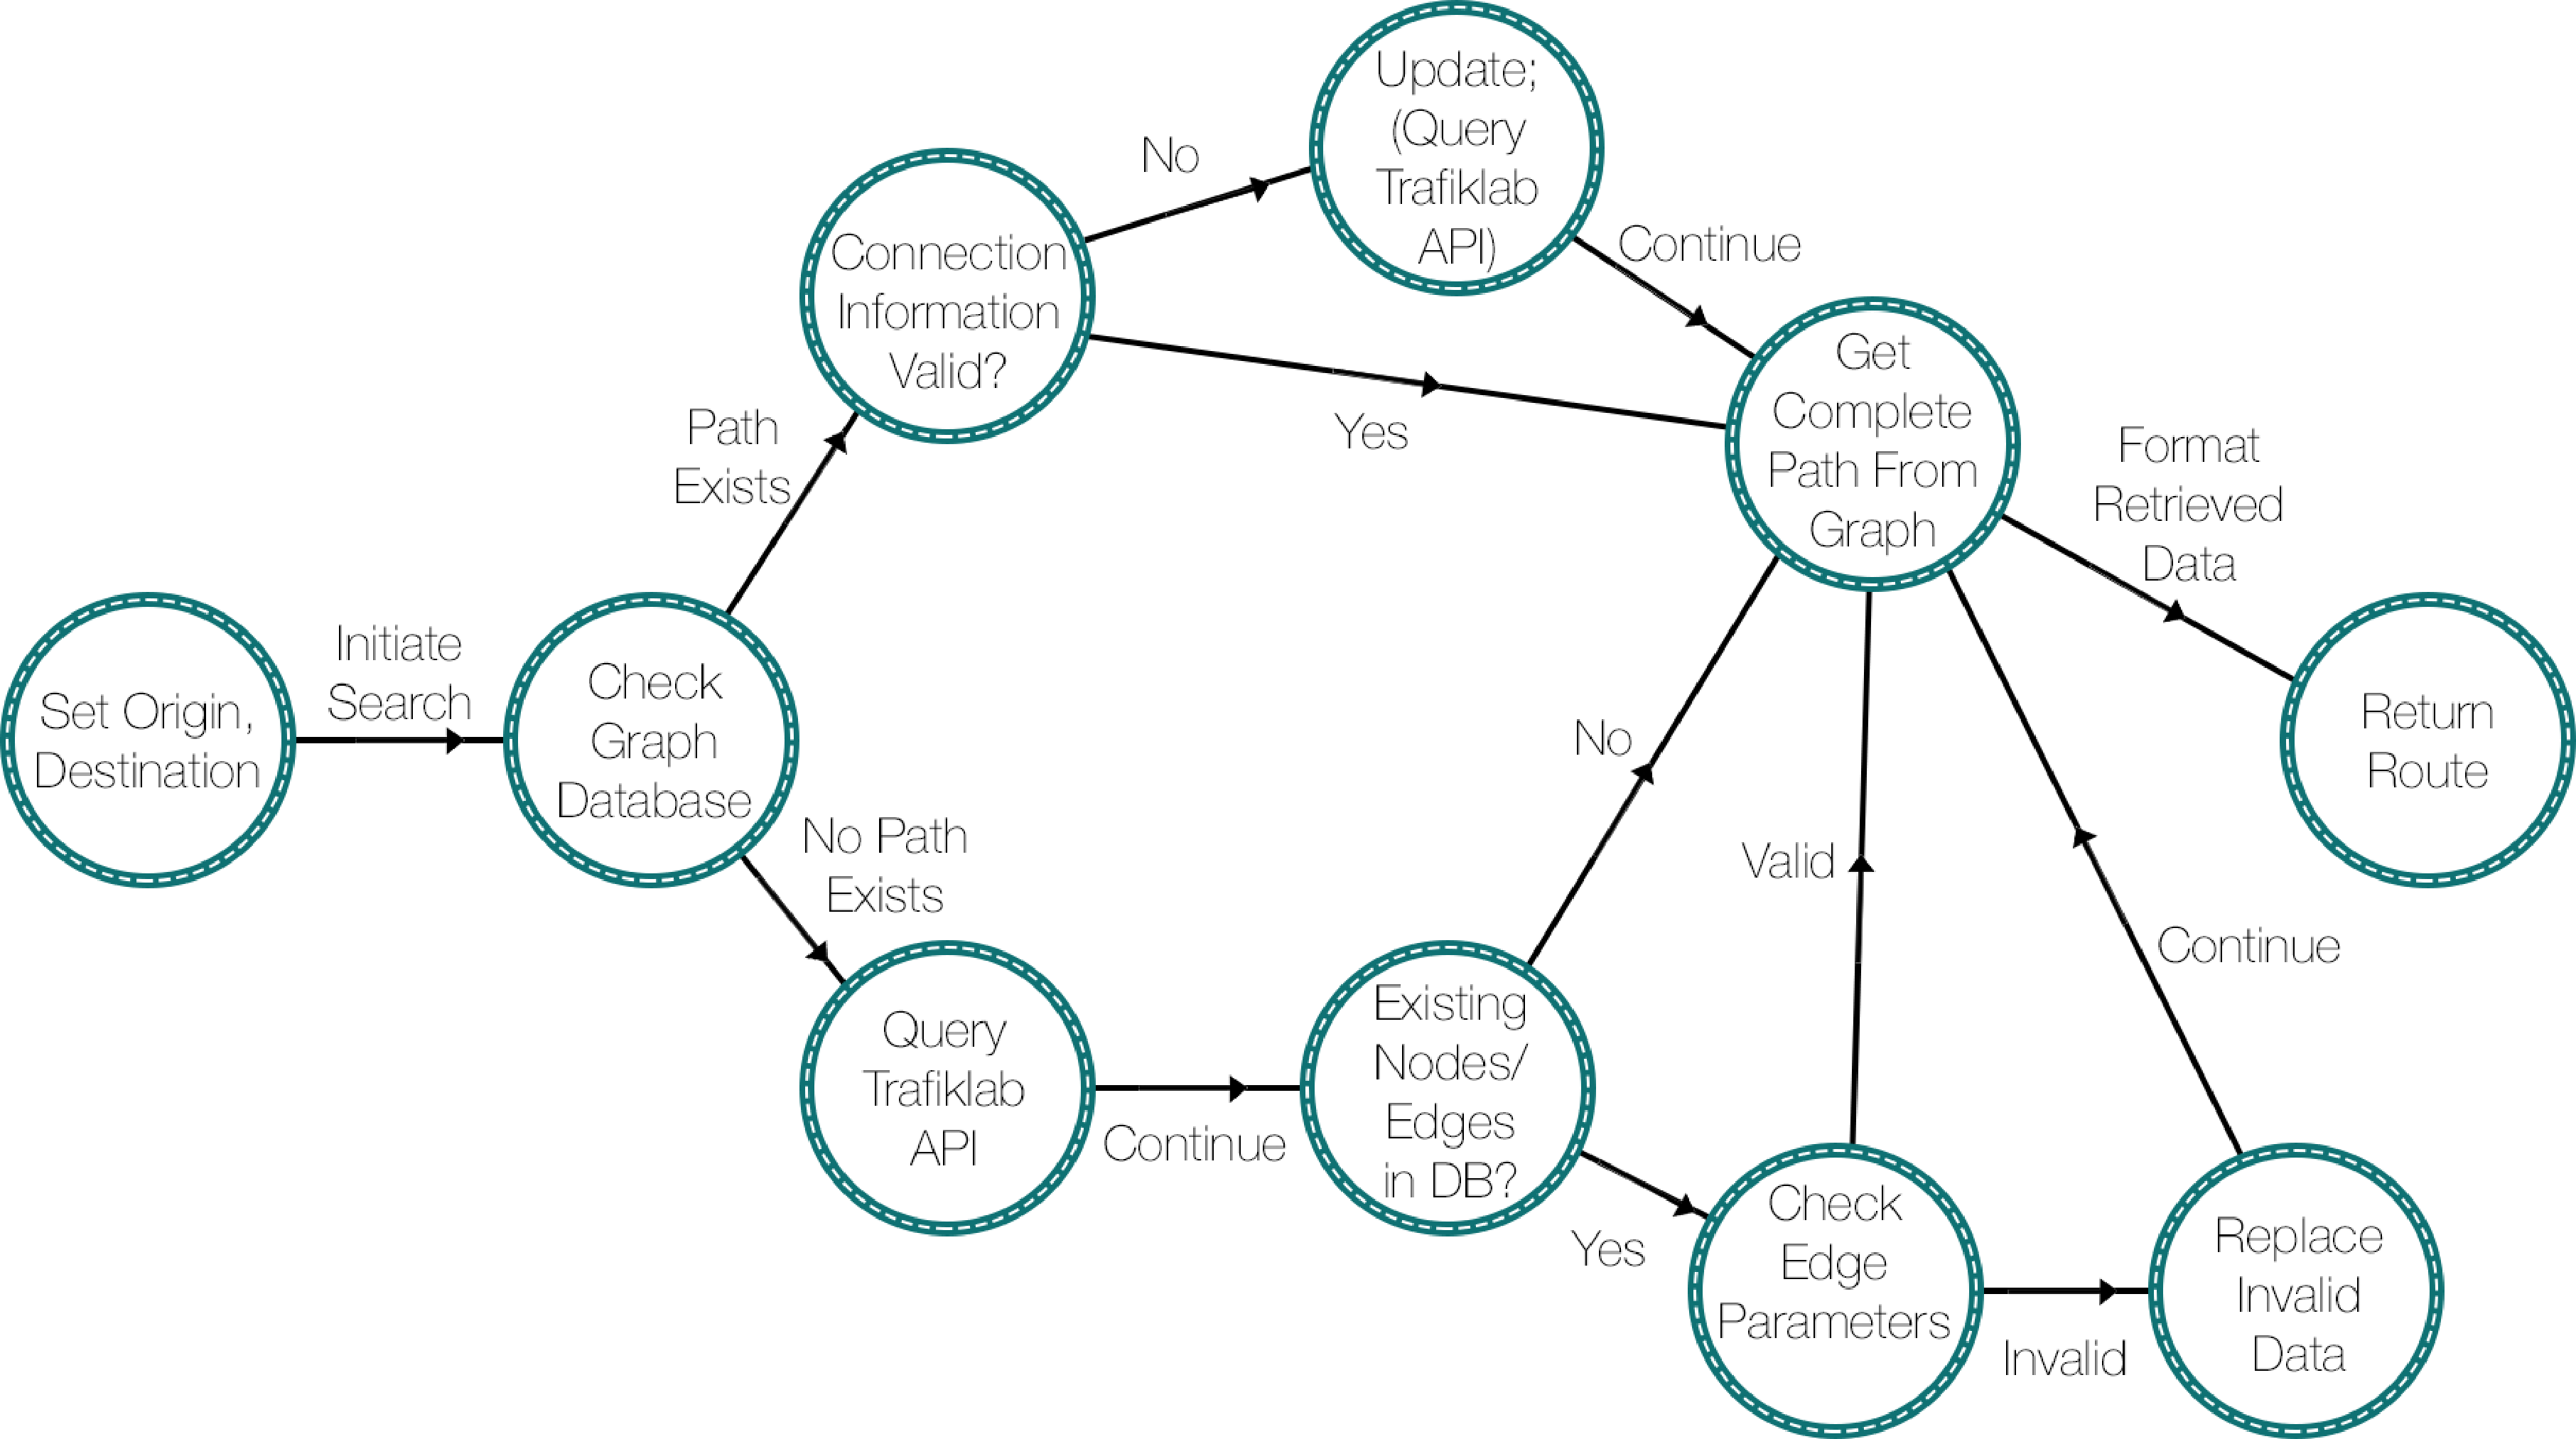
\includegraphics[angle=90, scale=0.3]{archoverview-nowhite-directed.pdf}}

\caption{Architectural Overview}
\end{figure}

\newpage

\subsubsection{Section A}
A check must be performed in order to determine if the origin location (Stop) node exists in the N4J GDB. The stop name, which is provided by the user, is stripped of any unsupported ASCII symbols, and the siteId for this stop name is found using the local JSON stop list reference. If the node (siteId) is present in the database continue to section D. If not, refer to section B. The siteId is used to check for the existence of the node in the database at this point, as the stopId identifier cannot be produced unless a TFLB Travel Planner API request is made. However, we attempt to avoid this unless there are no other available options.

\subsubsection{Section B}
It has been determined that the origin location Stop (node) does not exist in the GDB. A Travel Planner API request is mandatory, using the origin location and destination Stops that were previously set by the user. A JSON list containing the series of interconnecting stops (or a connection between two stops only) is returned from TFLB. Iterate over all indices of the list, assuming that more than one connection between two stops (this would simply be a direct connection between the origin and destination) exists. If a route can be mapped between these two locations from the TFLB API, continue. If not, refer to section C. Note that an index within this JSON list (returned by TFLB) will always contain an origin and destination.

The destination does not refer to the final required destination of the user if more than one JSON list index exists. Only the destination attribute of the last index will refer to the required destination. Intermediary stops, between the origin and destination, therefore, adopt this notation for the purposes of iteration. Basically, if a returned route is a list (intermediary stops between the origin and destination exist), the first index will contain the user defined origin, and the last index will contain the user defined destination. This is crucial information, as it allows us to establish relationships (edges) between the nodes in the GDB.

\noindent
\hfill
\begin{figure}[htp]
\centering{
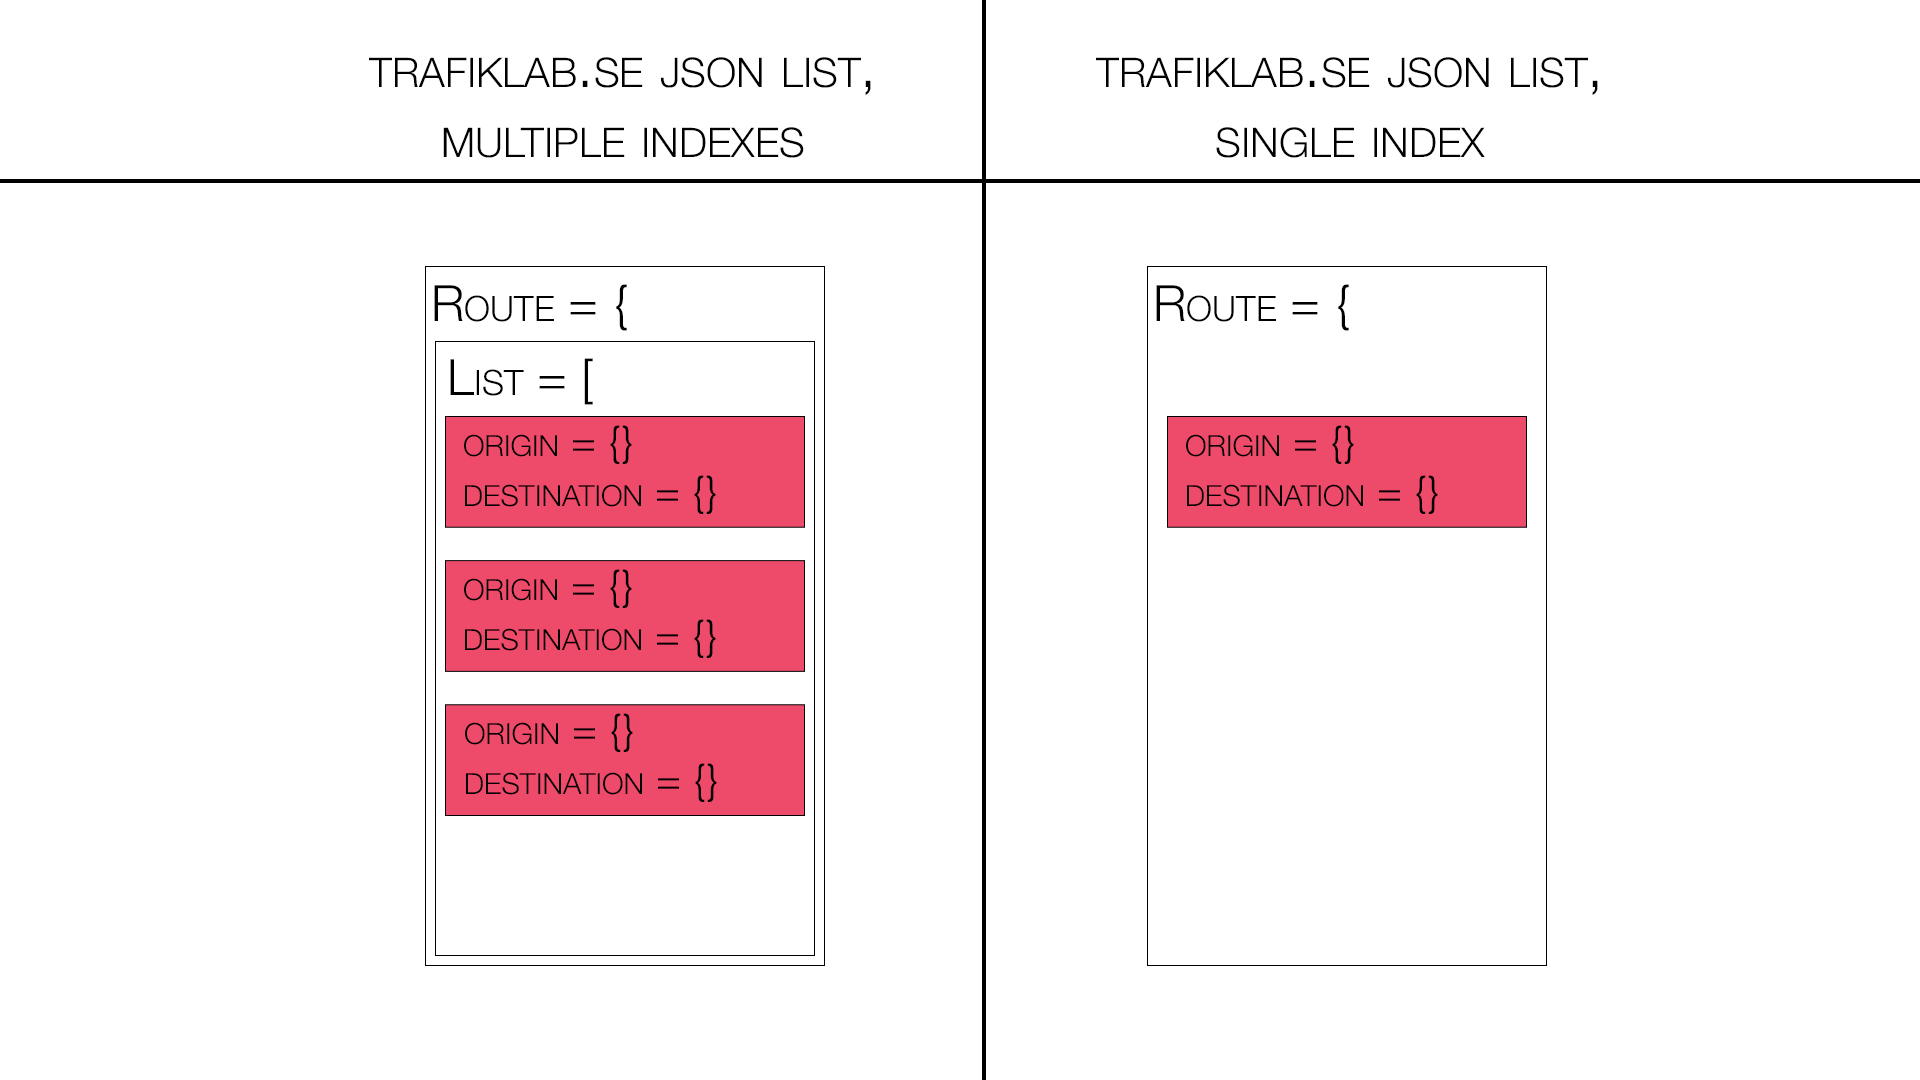
\includegraphics[scale=0.2]{stops-info.png}}

\caption{Stop information as returned by Trafiklab API.}
\end{figure}
\hfill

\noindent
TFLB ensures to add the indices to the JSON list in order of relevance to the route and never randomly populates a list. In order to determine if a stop node already exists in the GDB, we must check all current nodes in the list and compare the stopId parameter of the node to the “id” (within the JSON list) parameter of the current stop in the iteration. This stopId parameter is not represented in the graph as “id”, as an “id” parameter is already automatically assigned to each node by the GDB (defined above). If a match is found then the node already exists, and the system does not create a new node. If a match is not found then the node is created by the system with the appropriate parameters. The “id” parameter of the JSON list is renamed as the stopId of a node in the GDB.

Each relationship (GDB edge) contains four parameters. These include: i) id (assigned automatically by the GDB - this will not be referenced for the purposes of this project), ii) distance (referring to the distance between two stops (nodes) linked by the current edge), iii) departureTime (associated with the origin stop (node) added to the database for each index of the list - the destination stop cannot have a departureTime, this is impossible) and iv) departureDate (again, this is only associated with the origin stop node for each relationship in the connection of stops in the database).

We now examine the case that a route is returned by TFLB containing only one index. This index is not encapsulated by a list. Therefore, a direct link between the user defined origin and destination can be established. This origin stop (node) is added to the GDB. The system must now determine if the destination stop already exists in the GDB. The stopId parameter of the node is compared to all other stopId parameters in the list (should any exist). If a match cannot be found, the node is created and added to the GDB. A relationship (edge) is established between these two nodes. If a match is found, a connection is established between the newly created origin node and the pre-existing node. If a connection already exists between these two nodes then it must be validated by confirming that the train has not left the station or that the date has not expired. If invalid delete the relationship (edge) and create a new relationship between these two nodes. Otherwise, continue on. The results are then returned to the user and displayed on the appropriate web page.

We now examine the case that a route is returned by TFLB containing two or more indexes of stop to stop information incorporated within a JSON list. Each index of the list must be examined upon iteration. The origin within the initial index can instantly be added to the list, but the destination must be checked to ensure that a duplicate node is not created and inserted into the GDB. A relationship must be created between the origin and destination nodes. From this point onwards, all origin and destination stops for every index must be checked before a node (representing a stop) is created and inserted into the N4J database. A relationship (edge) between each of these origin and destination stops must be modelled, once they have been formally recognized within the GDB, and within each index. If neither stop exists as a node, create both nodes and form the relationship (edge). If one or both nodes already exist, simply form the relationship if one does not exist. If a relationship (edge) exists, check the departureTime parameter to ensure that it is valid (discussed above). If valid then continue,and  if not, update the relationship (edge). The results are then returned to the user and displayed on the appropriate web page.

\subsubsection{Section C}
A route cannot be generated by TFLB using the user defined origin and destination locations. This error is appropriately logged by the system, returned to the user and displayed on the appropriate web page.

\subsubsection{Section D}
A check must be performed in order to determine if the destination location (Stop) node exists in the GDB. The stop name, which is provided by the user, is stripped of any unsupported ASCII symbols, and the siteId linked to this stop name is found using the local JSON stop list reference. If the node (siteId) is present in the database then continue to section F. If not, refer to section E.

\subsubsection{Section E}
Please refer to section B. The required steps are similar, except that check prioritization is now associated with the destination stop as opposed to the origin stop. The results are then returned to the user and displayed on the appropriate web page.

\subsubsection{Section F}
The origin node siteId and destination node siteId exist in the GDB. It must now be determined if a one way directional relationship exists between the origin and destination stops (nodes) within the GDB. In order to determine if a connection between these nodes exists we must retrieve the shortest possible path through the measurement of the “distance” parameter assigned to each edge connecting two nodes in the graph. This is achieved with the application of Dijkstra’s Algorithm (defined in the Literature Review section) to the GDB. If the shortest path can be found then continue to section H. If not, refer to section G.

\subsubsection{Section G}
The shortest path between the origin and destination nodes using Dijkstra’s Algorithm cannot be constructed. This means that such a path simply does not exist, and a request to the TFLB Route Planner API is mandatory. The returned JSON list must be handled in the same manner as outlined in previous sections. The results are then returned to the user and displayed on the appropriate web page.

\subsubsection{Section H}
Ensure that the departureTime parameter of the edge connecting the origin node and the next node in the sequence (this may be the destination node, should only one connection exist) of the route is up to date.

If the departureTime of the connection has not yet occurred, and the departureDate of connection parameter matches the current date of the system, or has not yet occurred, then this route is considered valid and is returned to the user.

If the departure time has already occurred when compared with the current time of the system, but the departureDate parameter of the same connection does not match the current date of the system, another check must be performed. If the departureDate parameter of the connection has not yet occurred, then this route is considered valid and is returned to the user.

If the departure time has already occurred when compared with the current time of the system, and the departureDate parameter of the same connection matches the current date of the system, then this route is no longer valid and should not be returned to the user. Instead, a request to the “Travel Planner” API must be sent, and this new route returned to the system. The old route will be deleted, and replaced with this updated route. It is important to note that the nodes of the GDB are never deleted; only the relationship between them is removed should the above check fail. This relationship is then updated with the new information retrieved from the TFLB API request.

All other scenarios involving this connection are considered invalid, and a new route must be requested by the CPCS from the TFLB API. The new data should replace the older data where appropriate, and should only then be returned to the user.

\subsection{Design and Edge Direction}
A directed graph is a set of nodes that are linked together by a series of relationships (referred to as edges), where all of these edges are directed from one node to another.

It is very important to highlight that the series of relationships (or relationship if only one connection exists) between the origin and destination nodes, and all other nodes that make up the desired route are directional. For example, a journey from Marsta to Sigtuna is not the same as a journey from Sigtuna to Marsta. The methods of transport at a given time may be the same, but are definitely not the same train or bus (or some other method of transportation) as this is impossible. Essentially, the same bus or train cannot leave at the same time on the same date from two different locations. Therefore, if a journey exists from Marsta to Sigtuna, this is not an indication that the inverse of this journey is automatically true. Let us assume that a route from Marsta to Sigtuna exists in the GDB, but not the inverse of this journey. If the edges (connections) between the nodes (stops) of the route were not directed, then the system would regard both routes as the same journey and a user requesting information about a journey from Sigtuna to Marsta would be presented with the Marsta to Sigtuna route, which is completely incorrect.

\noindent
\hfill
\begin{figure}[htp]
\centering{
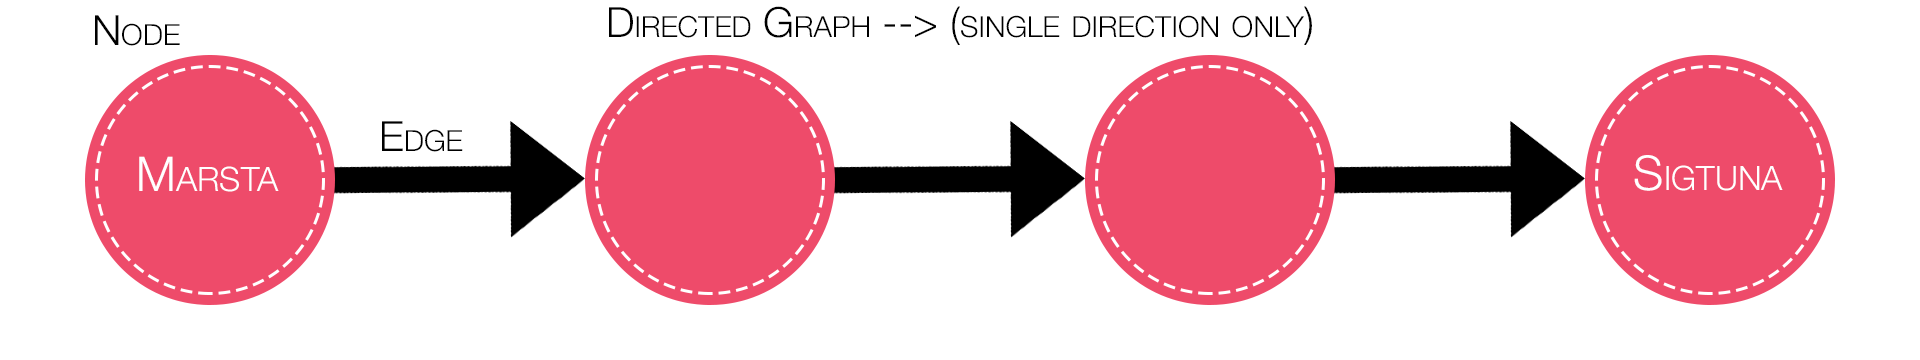
\includegraphics[scale=0.2]{directed-graph-2.png}}

\caption{Alternative Sample Route Data mapped within the GDB.}
\end{figure}
\hfill

\newpage

\subsection{Graph Database Cache Eviction Policy}
The GDB, particularly when applied to an application with a large user base, is constantly removing older connections that are no longer valid. A connection within some route is invalidated if one of the following criteria is satisfied: i) the departureTime parameter of the connection is invalid, ii) the departureDate parameter of the connection is invalid, iii) the method of transport or service is no longer available or has been cancelled (cancellations are managed by TFLB) or, finally, iv) if another route is required to make use of the same connection, this connection, even if still valid, is updated when a fresh query to the TFLB API is requested.

If any of the above criteria are satisfied, then an eviction is required. This means that the connection (the edge within the GDB) between two nodes is removed and a new connection is then established with updated inter-stop (node) relationship parameters.

\newpage

\subsection{Manipulation of Requested Trafiklab Information}
SL Location Lookup [25] is used to retrieve the siteId of any named stop (a stop name could be “Arlanda”, for example) within the SL [23] database, and which a user can access via the TFLB open API. The API is then queried for the appropriate data, not the actual SL [23] database, as this is not available publically. This siteId is used to check for the existence of a stop node in the GDB. Information is returned in JSON format.

SL Stops and Lines 2 [26] is used to map each and every stop to a set siteId (set by SL, and accessible via the TFLB open API). This siteId remains static and this dataset of stops is regularly maintained, but rarely updated with new stops (as is evident by the date of the most recently added stop), and therefore is a suitable anchor for our database existence checks. To save time, this data is requested manually once per week, and the most updated version is stored locally within the project directory. Expenses are reduced, as an API request is not without charge. This data must be requested for not only the origin and destination stops set by the user, but also for every stop linking these two points when a Travel Planner API request is made. These stops must be stored in the GDB with a stopId and siteId assigned as reference identifiers for accessibility purposes. Therefore, it is evident that running costs will rapidly accumulate without the local storage of this data. Information is returned in JSON format.

SL Trip Planner 2 [27] is used to generate a route between the user defined origin and destination locations. Important information retrieved from this API call include: i) stopId, ii) departureTime, iii) departureDate, iv) stopLatitude, v) stopLongitude and vi) the stopId (not the siteId - these are completely different parameters, and the significance of which is defined in more detail in the design section of this document). The relevance of each of these parameters is discussed in later paragraphs within this section. Information is returned in JSON format.

All data returned in JSON format must be returned in a similar manner. For example, the manner in which this data is accessed must be static, otherwise the CPCS will constantly yield “KeyError” python errors. The CPCS cannot access JSON information, or any information for that matter, that does not exist. However, TFLB ensure that all data returned is routinely structured. Once it was determined that the manner in which data is returned would not alter, it was necessary to construct methods (functions) that would accurately index and access the data returned from the API. This ensures that the information can be used with other features of the system.

In many instances, due to the nature of the data retrieved, stop names are presented in Swedish. The Python programming language does not recognize many Swedish language symbols. In order to circumnavigate this issue, all stop names are assigned to a Python variable so that they can be stripped of any and all unrecognized ASCII symbols. The same methodology is applied to the aforementioned local JSON list of stop names which yields a corresponding siteId. User defined origin and destination locations, as well as every stop within a route generated by the SL Travel Planner (Trafiklab, SL Travel Planner) must adhere to this rule.

The Haversine formula must be used to find the distance between two stops. This takes the latitude and longitude coordinates, which reside on the surface of the planet, of both the origin and destination stops as parameters and return the straight line distance between the two points. The issues surrounding the usage of the Haversine formula for the purposes of this project are outlined in the Literature Review section of this document.

Data returned from TFLB can be iterated in two ways and is accessible via two loops, an outer loop and an inner loop. The former encapsulates the latter. The outer loop yields the number of upcoming routes within a time period that can be managed by TFLB, or overwritten by the system administrator. The default settings remain unaltered for the purposes of this project. The inner loop yields the number of stops for each route.

\newpage

\section{Implementation and Evaluation}
\subsection{Brief Overview}
The backend of the web application was created using Python, managed by a model-view-controller (MVC) architectural pattern. Information and user input for any actual web page is governed by html. Aesthetic presentation of the aforementioned display data is controlled by CSS and Bootstrap [3]. The Integrated Development Environment (IDE) Pycharm [19] effectively groups the sizeable code into manageable segments for maintenance and upgradability purposes.

The GDB was constructed using N4J. P2N is employed for the seamless integration of N4J and Python. Nodes and Edges are inserted as required, and the web application manages the edge direction between all nodes where applicable. All information, such as stop names and edge parameters, is stored in the GDB as standard ASCII strings, and data is retrieved using the Cypher Query Language.

Graph nodes and the connections that exist between them, where relevant, are monitored using the supplied graph visualisation tool. This application feature presents the contents of the N4J GDB in an aesthetic manner, which is particularly useful for verification and analysis of the data. Restrictions are permissible, and are applied to the data using the provided user interface taking into consideration the following: i) number of nodes that can be displayed, ii) choosing the size and color of the differing node types (where relevant) or iii) simply selecting edges that conform to one direction.

User input is handled by the web application. It is captured by a segment of Javascript, and posted to the server so that a route may be constructed. All results are presented to the user upon redirection when the user selects a “Search” button. The web application also provides support for mobile and tablet users, where the sizing parameters are controlled by the Bootstrap [3] and CSS regulations.

\subsection{Required Software and Applications}
The following section describes the tools used to construct the system, and explains the way in which they were used, why they were necessary and how they are relevant to the title of the document.

The system is developed and maintained using the 64-bit Linux distribution Ubuntu [28]. The operating system version is 16.04 LTS (Xenial Xerus).

Virtualenv (or venv), is used to manage the versions of all other tools used in the project. It is imperative that versions of all tools remain static, until otherwise specified by the system administrator. This will prevent errors when newer versions of tools are updated and existing methods are marked as deprecated by the product managers.

Python is the programming language applied to construct the backend of the system. Python supports many standard system libraries, and several were used. These are defined under a separate heading and listed below. This language was chosen for many reasons: i) Xerial Xenus (the Operating System) natively supports Python, ii) comprehensive documentation and support, iii) personal familiarity with the language, iv) support for GDB drivers such as P2N, which is defined below, and v) for ease of management of external python tools and libraries through the use of virtual system environments. Python version is 2.7.13.

The system was largely developed and tested using the command terminal supplied by Ubuntu. However, as more features were incorporated, the data could not be contained within a clean and concise frame. Therefore, a web application was constructed using the python web framework Django [9]. Django was chosen for the following reasons: i) comprehensive documentation, ii) secure network request management system (required for distributed access to the GDB by multiple machines) and iii) support for external format structuring tools, format styling tools (CSS, Bootstrap [3]) and interactive effect management tools (Javascript). Django version is 1.10.5.

Hypertext Markup Language (HTML) is a standardized system for tagging text files to achieve font, colour, graphic, and hyperlink effects on all web pages displayed to the user by the proposed system. HTML version 5 is used.

CSS presents the returned route information to the user in an aesthetic manner, allowing for the design of a user-friendly interface. Bootstrap [3] provides custom CSS templates and html tags used to split up sections of the page, enabling uncomplicated page styling and feature positioning. Bootstrap [3] version 3.3.7 is used.

Interactive effects on each web page such as drop down lists, user input manipulation and bilateral data visualisation are all achieved through the use of Javascript.

N4J is a GDB that displays all defined nodes and the connection between any or all of these nodes, should such a relationship exist (edges). The system administrator must specifically define the format of these nodes and edges (the given name, and all other attached properties). Nodes and edges, by default, are given a unique identification number (id) upon creation so that, upon query, they can be easily identified and managed. The nodes and edges are managed in the sense that they can be removed or updated by N4J, through the use of Cypher (defined below), the N4J database query language . N4J was chosen as it provides comprehensive documentation, a natively supported database query language and an aesthetic database visualisation tool in the form of a web app, accessible via the machine which manages the database. All created nodes and edges, if any, are prominently displayed by the web app, allowing for efficient data management and error handling. Nodes can be traversed using many methods. In this instance, the graph produced will be directed (i.e. all edges within the GDB are directed from one node to another), meaning that they can have a forwards or backwards facing relationship. For example, a stop can be connected to another when a bus links these two stops. This bus travels from the first stop to the other, therefore the relationship here is directional. However, it is also relevant to take into consideration the possibility that the bus can also return from the destination stop to the original stop. A new relationship is created, but it is of the opposite direction of the first relationship. This means that multiple relationships between nodes can exist with opposing directions (where relevant).

\noindent
\hfill
\begin{figure}[htp]
\centering{
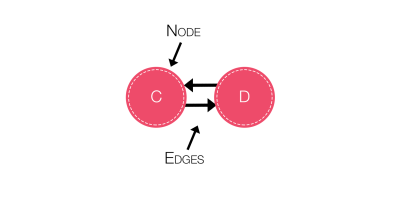
\includegraphics[scale=0.6]{multi-dir.png}}

\caption{Two nodes with multiple connections in opposing directions.}
\end{figure}
\hfill

P2N is a N4J driver for the Python programming language. P2N is used as it enables seamless integration of the N4J database query language, Cypher, and the Python programming language. This allows for more concise Cypher queries. Actual Cypher queries are also supported where required. P2N version is 2.0.9.

Cypher is the N4J database query language. It can be used within the provided N4J Cypher console, or as a query directly within a python script. There are no other options available that grant the same level of N4J database management operations. Cypher is comprehensively documented.

Git [11] is the version control system used to manage changes made to the codebase. GitHub [12] is the remote repository where all project files are stored.

Pycharm is used to develop and maintain the CPCS. This is an Integrated Development Environment (IDE) specifically designed for python, with native support for external plugins which enable modification of other file types within the same project. Pycharm highlights errors within the codebase such as indentation errors, spelling errors and incorrect method references. The IDE also synchronises well with git, but this feature was not utilized for the purposes of this project. Pycharm version is 2016.3.

\subsection{Technical Challenges - Design Suitability}
Most importantly, it was determined that it is very straightforward to represent and visualise stops and their relevant connections as nodes and edges in a GDB respectively. TFLB route information to GDB representation, as a result, is easily managed. TFLB also manages route data using the route, leg, connection storage mechanism, allowing the CPCS to manipulate and store data with respect to the manner in which the information is presented without the prerequisite of journey “leg” reordering.

Connections between stops, represented as edges in the GDB, reference all information for a specific method of transport. This includes departure and arrival times, distance and location. When a connection (edge in the GDB) becomes invalid, it is simply a matter of removing the connection so that it can be replaced, or updated in certain instances. The stops (the nodes of the GDB) are never removed. Only the connections between them (if any) are regarded as valid or invalid. If invalid; query TFLB. If valid then return the immediate information which will result in a massive performance improvement (refer to the Results section of this document).

As mentioned previously, the design of this directed graph implementation was inspired by the Google Knowledge Graph.” Querying the graph for data that shares similar characteristics, on a regular basis, is more efficient than using a traditional relational database such as MySQL (see Literature Review section).

One major disadvantage associated with this type of design is the amortised cost effectiveness analysis with respect to systems (CPCS) that do not query similar data from the GDB on a regular basis. This is due to a small user base. Information must be requested from TFLB when a route does not exist in the GDB, and a complete path cannot be constructed from a series of partial paths. This means that the total time for a request is the time to query both the GDB and the TFLB API, but the route now exists in the GDB. If this route is requested again, while valid, then query time is reduced as the time to query the TFLB API is far greater (see Results section). However, if the data is not queried while this same connection is still valid in the GDB, then the total amortised time is much greater overall as the potential performance gains of avoiding a TFLB API request are never realised.

\newpage

\subsection{MVC Architecture}
The MVC design pattern ensures that objects within an application (the CPCS) are assigned one of three roles: i) model, ii) view and iii) controller. The model represents the underlying business logic of the application. No information is contained regarding the user interface. The view is the collection of classes representative of the elements which construct the user interface. Finally, the controller is made up of the series of classes which connect the model and the view. It is possible to communicate between the classes of the model and the view using the controller.

Another technically challenging aspect of this research topic was the deployment of a version of the CPCS which utilized the MVC design pattern. This architectural design choice ensured that any route decisions determined by the CPCS would be contained within a single application. Although the construction of such a system was not a straightforward task, it ensured that all required tests could be undertaken without major complications. Finally, the most important aspect of a modular MVC approach to the problem ensures that the CPCS is reusable for any other future potential system administrators [16] who wish to modify the system for personal use.

\noindent
\hfill
\begin{figure}[htp]
\centering{
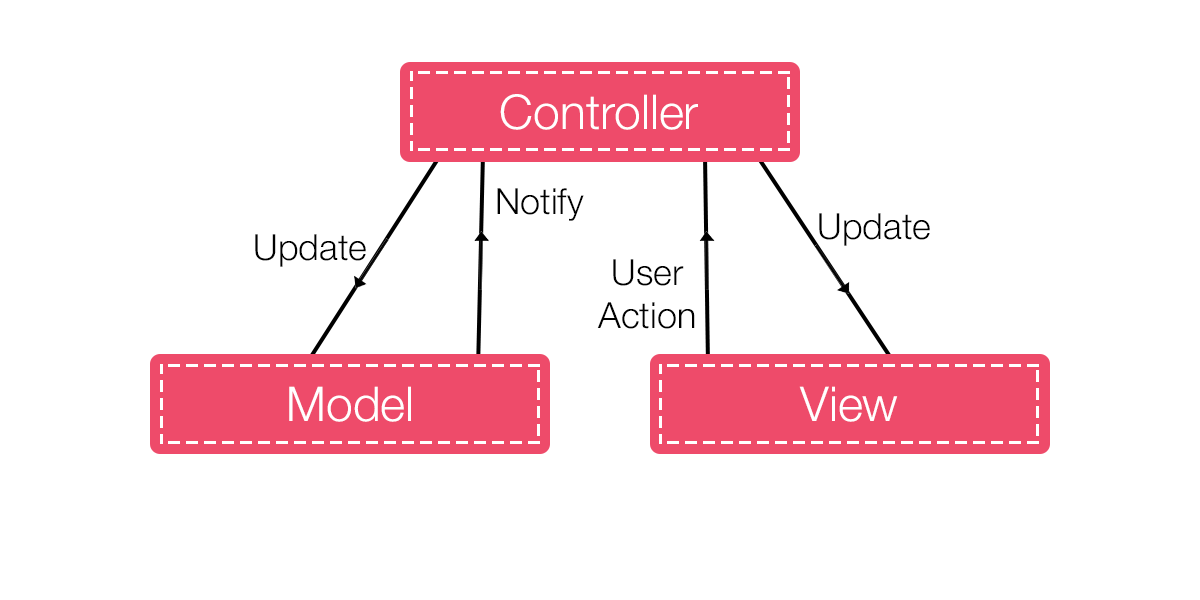
\includegraphics[scale=0.2]{mvc-diagram.png}}

\caption{MVC architectural overview.}
\end{figure}
\hfill

\newpage

\section{Results and Conclusions}
This section presents all findings and test results. It also refers to the initial objectives: i) performance improvement, ii) cost reduction (with respect to bandwidth and processing power in particular) and iii) aesthetic result presentation upon demonstration of all results. Graphs, images and other reference materials are labelled appropriately.

\subsection{Analysis}
Results are tested through the use of the CPCS, the GDB and the TFLB API. They reveal that the construction of complete paths from partial paths, when applied to this system, solve the three primary issues outlined at the beginning of this section.
	
Furthermore, it can be deduced that for large scale systems, the performance improvement through the reduction of the time taken to complete a route search for all users of the system scales exponentially, and factors into consideration the amortized cost of a search. This deduction is based on the analysis of the produced performance metrics, and the time taken to request the TFLB API data.

\noindent
\hfill
\begin{figure}[htp]
\centering{
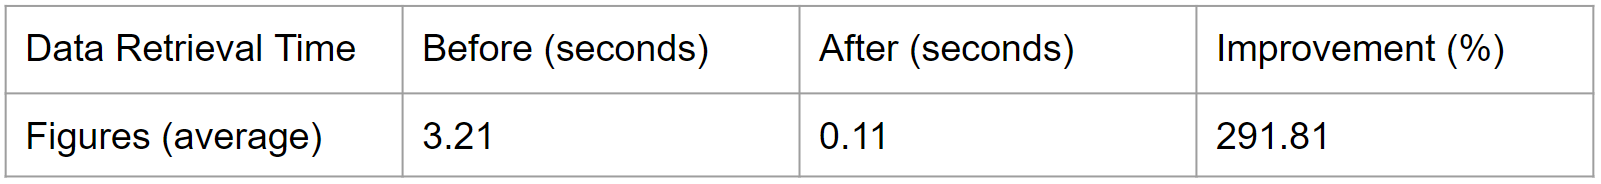
\includegraphics[scale=0.3]{performance-gains.PNG}}

\caption{Screenshot of actual CPCS performance improvement.}
\end{figure}
\hfill

\noindent
With respect to the figures presented in the above image, it is evident that a significant performance increase has been achieved as a result of the construction of the CPCS. The average time taken to retrieve a route from TFLB is 3.21 seconds. This result was calculated by manually recording the time taken to retrieve data from the TFLB API over 50 individual scenarios. It was imperative to also ensure that any TFLB API did not already implement some form of caching for queries within a certain time period. The total time taken was recorded by initialising a timer within the Python code immediately before the first necessary TFLB API query. The timer was then halted immediately after a route had been found, or not found in some instances, if such a route did not exist.

The time taken to construct a route was also recorded in the same manner in the event that the GDB was traversed, a result was found and a query to the TFLB API was not required. The average of 50 manually tested scenarios, 0.11 seconds, was recorded.

Therefore, it can be decuded from these results that a significant average performance increase of 291.81\% is achieved. Similarly, the major factors of cost reduction, processing power and bandwidth, have also been addressed. Total required processing power is reduced, as only a query to the GDB must be made, and not a query to the GDB and the TFLB API combined. A specific scenario outlining an example of such a series of tests is outlined in the following paragraph.

It is relevant to reiterate that the amortized cost is the total time saved when a route is initially stored in the GDB following a request to the TFLB API, then requested at least once more before the route is invalidated. An example includes the train (transport method of particular edge within the GDB) leaving the station. In the event of only one user requesting a certain route, constructed from partial paths or immediately available, then the amortized cost of this search is effectively zero, as no user has capitalized on the potential query time reduction by retrieving information from the GDB alone.

\noindent
\hfill
\begin{figure}[htp]
\centering{
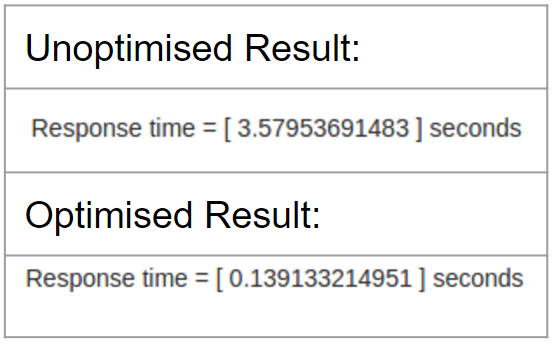
\includegraphics[scale=0.4]{response-time-diff.PNG}}

\hfill

\caption{Screenshot of potential optimization percentages. Results are captured from the CPCS.}
\end{figure}
\hfill

\newpage

\noindent
Below is a screenshot of the home web page where users of the CPCS can search for a route using the origin and destination input sections:

\noindent
\hfill
\begin{figure}[htp]
\centering{
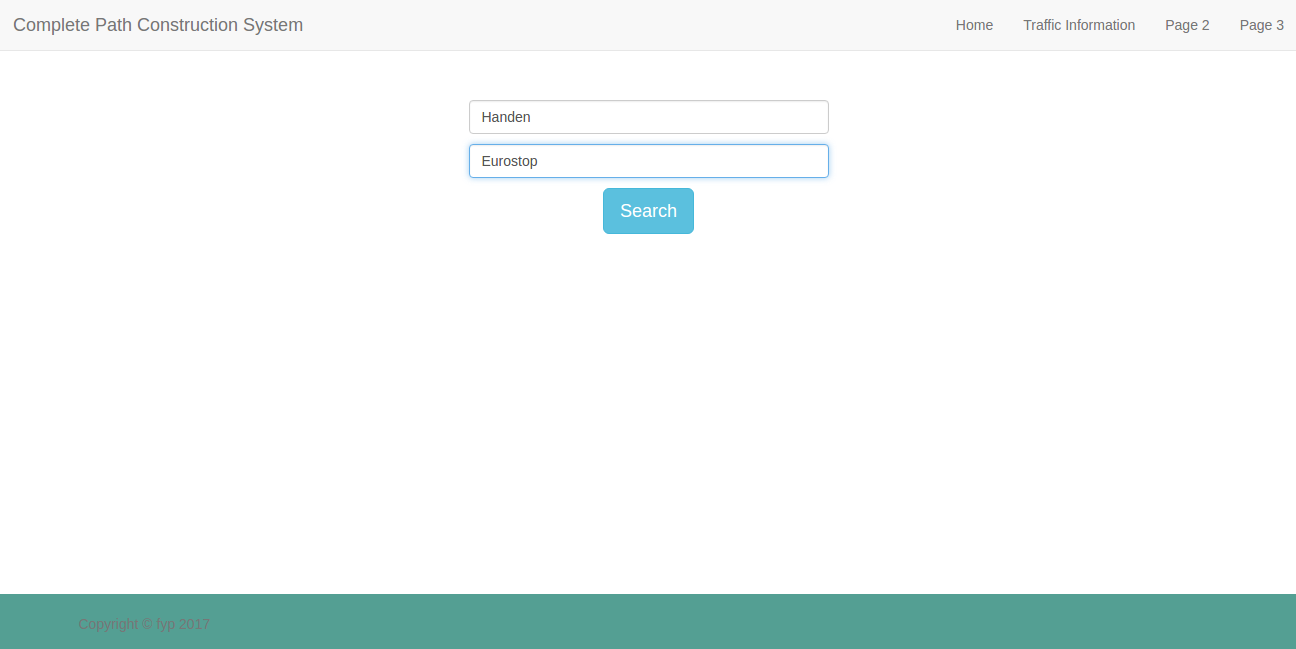
\includegraphics[angle=90, scale=0.35]{CPCS-home.png}}

\hfill
\caption{Screenshot of the CPCS route search, home web page.}
\end{figure}

\newpage

The second major issue is cost reduction. It is analysed by gathering data highlighting the number of times the GDB (the smart cache) is queried and also the number of times that the TFLB API is queried. A query to TFLB is regarded as a charge, as the initial complimentary request allowances are ignored for testing purposes. The cost of a charge is irrelevant, as the focus of this section is primarily the total number of potential queries that could be made without a charge, as opposed to the actual amount saved for all queries combined.

\noindent
\hfill
\begin{figure}[htp]
\centering{
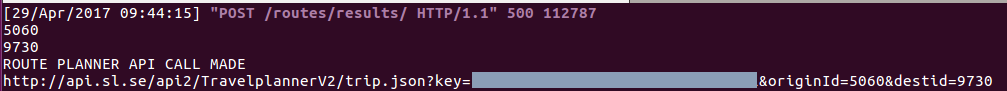
\includegraphics[scale=0.4]{cache-miss-blur.png}}

\caption{Screenshot of TFLB GDB cache miss.}
\end{figure}
\hfill

\noindent
Demonstration of the same request made 125 seconds later while the connection remains valid within the GDB:

\noindent
\hfill
\begin{figure}[htp]
\centering{
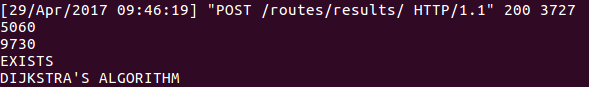
\includegraphics[scale=0.5]{cache-hit.png}}

\caption{Screenshot of TFLB GDB cache hit.}
\end{figure}
\hfill

The user interface is clean and concise, and displays only the most relevant information. This can be compared to the route information return style of TFLB, as the CPCS is far more comprehensive and it is evident that a basic JSON list is not the most appropriate manner in which to present meaningful response data.

\newpage

\begin{figure}[htp]
\centering{
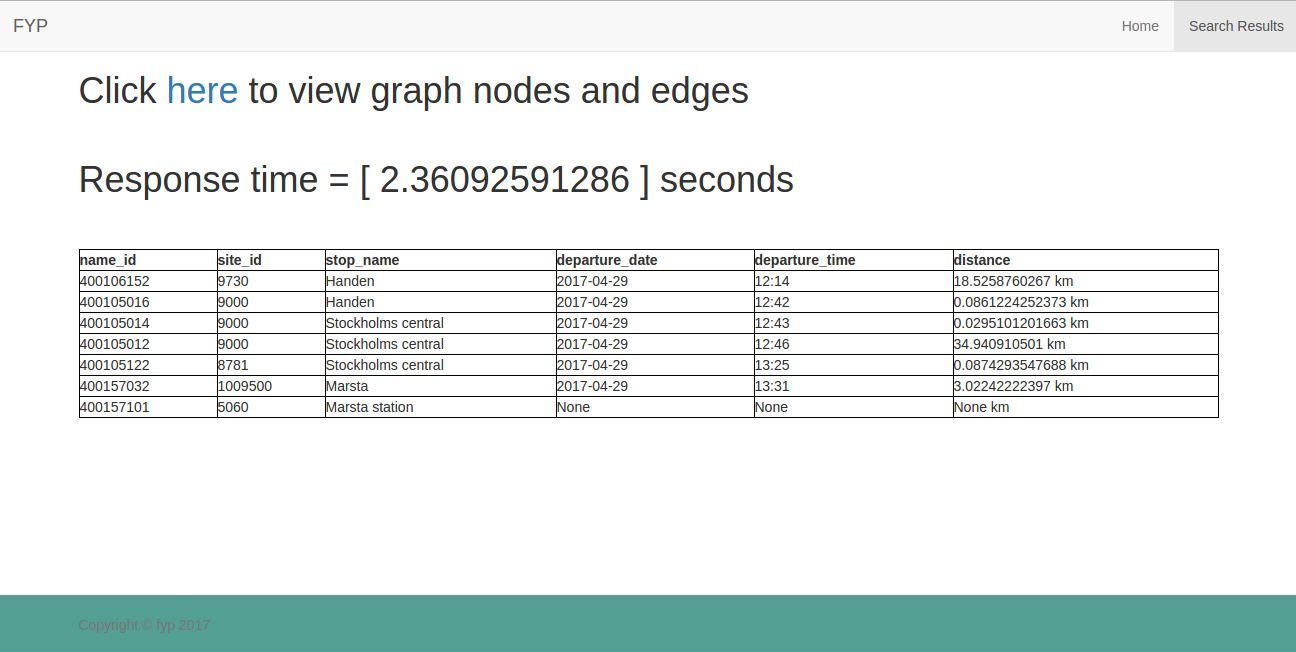
\includegraphics[angle=90, scale=0.29]{aesthetic-miss.png}}

\hfill
\caption{Screenshot of CPCS aesthetic presentation with cache miss.}
\end{figure}

\newpage

\noindent
The same CPCS response as above. This time the GDB has been successfully queried, and a TFLB API request is not required.

\hfill
\begin{figure}[htp]
\centering{
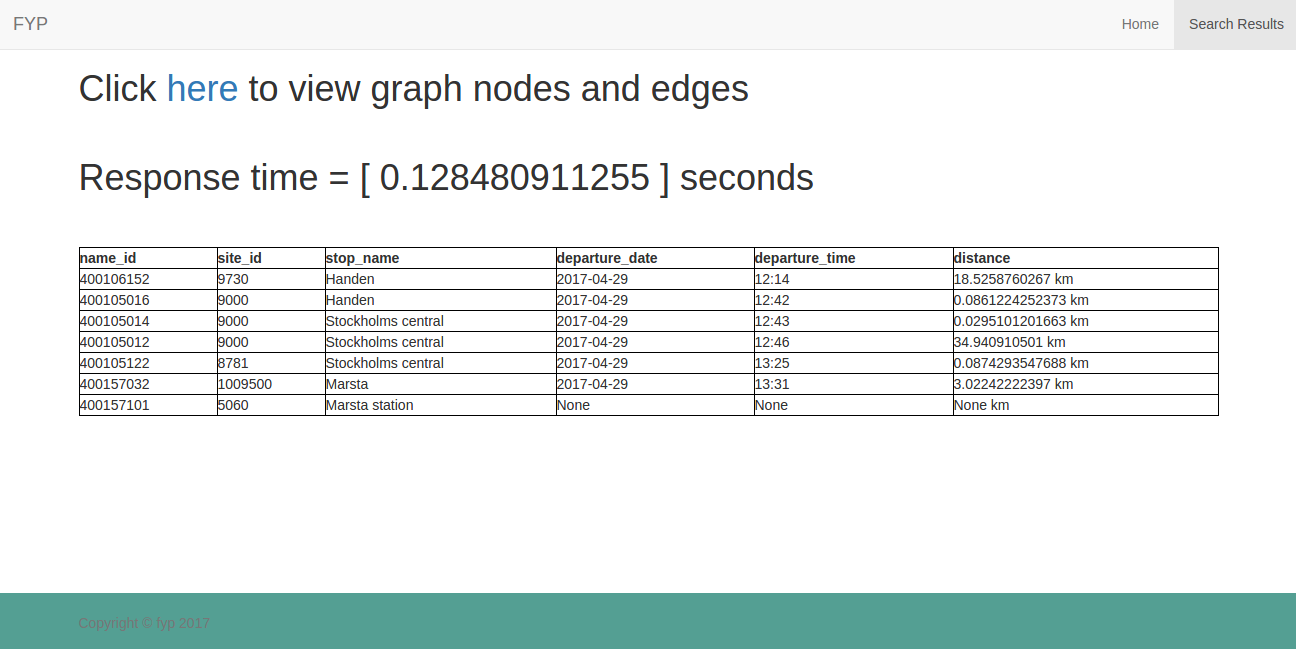
\includegraphics[angle=90, scale=0.29]{aesthetic-hit.png}}

\hfill
\caption{Screenshot of CPCS aesthetic presentation with cache hit.}
\end{figure}

\newpage

There are many improvements that can be made to the final product, and these are discussed in the Future Work section. A comparison between the initial prototype, the final product produced and other external sources of inspiration is also examined.

\newpage

\subsection{Concluding Remarks}
The final results suggest that the potential exists for a massive performance improvement to large scale systems similar to that of the CPCS. A complete test with a large volume of participants was not undertaken. Such a procedure was not a requirement, and was not categorized as a parameter of the overall scope of the study.

Furthermore, it can be derived that this web application will reduce system costs, as fewer queries to external APIs such as TFLB are required. As mentioned previously, such a query is not without charge. A partially replicated graph, through the bespoke caching of graph data, is an appropriate manner in which to resolve the problems presented in this document. Essentially, all data that is susceptible to graphing is considered favourable, as the resulting information derived covers the three main issues outlined in the Introduction section of this research topic.

It is evident from the results presented in this section that the CPCS is not just a simple route caching solution. A route which has not been specifically requested previously may be derived from the existence of alternative paths in the GDB if the direction of these paths is consistent with the direction of the route. In summary, if only the following paths, path A to C (A, B, C, D) and path B to E (B, C, D, E) exist in the GDB, then path A to E may be derived. Therefore, a request to the TFLB API is not required when querying for route information regarding path A through E, even though this path does not directly exist in the GDB. The overall design of the CPCS is representative of a complex, smart caching system. However, the suggested effectiveness of the CPCS is entirely dependent on the number of users of the system with respect to the amortized cost of a route search.

Overall, it can be concluded that the objectives of this research project have been achieved. There is still, however, wide scope for improvement and for further research. Future developments of the system, and general enhancements, are outlined in the following section.

\newpage

\subsection{Future Work}
At present, only one edge can exist in one particular direction between two nodes in the GDB. Multiple edges can exist between nodes in the GDB, provided that the direction of the edges are not the same. Future work will enable support for multiple, directed connections (edges) of the same direction between nodes. This enables additional user choice in terms of i) mode of transport selection, ii) price limitations and iii) timing selection.

Another development area is the improvement of the design of the route presentation (search results) web page. While functional, the overall aesthetics remain quite basic, but represent an improvement visually when compared with a standard JSON list.

In the future, the calculation of the total financial amount saved for a given time period will be necessary, as opposed to the present system of simply calculating the number of times a call to an external API has been avoided. This would include allowing a system administration to govern all the parameters around this feature.

Most importantly, it must be determined if the routes inserted into the GDB are actually the most effective. For example, let us imagine that there are two nodes within the GDB that are representative of two stops. The connection that exists between them is valid. However, it is possible that an alternative connection can be assigned. The departureTime parameter of this alternative connection is a later time than that of the current connection, but the arrival time is slightly sooner. Obviously, this alternative connection is more appropriate, but has not been assigned as a result of the later departureTime. However, this feature is not within the scope of this research topic, and therefore has not been addressed for the current implementation of the CPCS.

There are many other issues that can be resolved using this method of crowd (smart) caching. One such example includes matching developers and relative code preferences on GitHub in terms of preferred language, external application familiarity, and also with respect to the discovery of links between developers for role suitability. All information gathered would, in theory, establish some connection between individuals and their respective work which has been published to github so that the most suitable candidate for the future relevant occupation is found. This application of the GDB may prove to be an effective human-resources software solution.

\newpage

\section{Bibliography}
\begin{enumerate}

\item
Balcombe, R., Mackett, R., Paulley, N., Preston, J., Shires, J., Titheridge, H., Wardman, M. and White, P., 2004. The demand for public transport: a practical guide, 5(2), pp.39-40.

\item
Bondy, J. A., Murty, U.S.R. (1976). Graphs and Subgraphs. Graph Theory with Applications, 1(6), pp. 12-14.

\item
Bootstrap, 3.3.7, http://getbootstrap.com/, Accessed on 2017-03-29

\item
Brandes, U. (2001). A faster algorithm for betweenness centrality, The Journal of Mathematical Sociology, ch. 25, sec. 2, pp. 167-169.

\item
Caughman, J.S. and Veerman, J.J.P., 2006. Kernels of directed graph Laplacians. the electronic journal of combinatorics, 13(1), p.R39.

\item
Chang, F., Dean, J., Ghemawat, S., Hsieh, W.C., Wallach, D.A., Burrows, M., Chandra, T., Fikes, A. and Gruber, R.E., 2008. Bigtable: A distributed storage system for structured data. ACM Transactions on Computer Systems (TOCS), 26(2), p.4.

\item
Chung, Y.C. and Ranka, S., 1992, December. Applications and performance analysis of a compile-time optimization approach for list scheduling algorithms on distributed memory multiprocessors. In Proceedings of the 1992 ACM/IEEE conference on Supercomputing (pp. 512-521). IEEE Computer Society Press.

\item
Dijkstra, E.W., 1959. A note on two problems in connexion with graphs. Numerische mathematik, 1(1), pp.269-271.

\item
Django, 1.10.5, https://www.djangoproject.com/, Accessed on 2017-03-29

\item
Drukker, D.M., Peng, H., Prucha, I.R. and Raciborski, R., 2013. Creating and managing spatial-weighting matrices with the spmat command. Stata Journal, 13(2), pp.242-286.

\item
Git, 2.7.4, https://git-scm.com/, Accessed on 2017-03-29

\item
Github, https://github.com/, Accessed on 2017-03-29

\item
Google Maps, Release 3.27, https://www.google.ie/maps, Accessed on 2017-04-26

\item
Haigh, M.S. and Bessler, D.A., 2004. Causality and price discovery: An application of directed acyclic graphs. The Journal of Business, 77(4), pp.1099-1121.

\item
Have, C.T. and Jensen, L.J., 2013. BIOINFORMATICS EDITORIAL. Bioinformatics, 29(24), pp.3107-3108.

\item
Krasner, G.E. and Pope, S.T., 1988. A description of the model-view-controller user interface paradigm in the smalltalk-80 system. Journal of object oriented programming, 1(3), pp.26-49.

\item
Miller, J.J., 2013, March. Graph database applications and concepts with neo4j. In Proceedings of the Southern Association for Information Systems Conference, Atlanta, GA, USA (Vol. 2324, p. 36).

\item
Neo4j, 3.1, https://neo4j.com/docs/, Accessed on 2017-03-29

\item
Pycharm, 2017.1.1, https://www.jetbrains.com/pycharm/download/, Accessed on 2017-04-24

\item
Python, 2.7.13, https://docs.python.org/2/, Accessed on 2017-03-29

\item
Py2neo, 2.0, http://py2neo.org/2.0/cypher.html, Accessed on 2017-03-29

\item
Rodriguez, M. A., Neubauer P. (2010). The Graph Traversal Pattern. Graph Data Management: Techniques and Applications. pp. 38-43.

\item
SL, Latest Release, http://sl.se/, Accessed on 2017-04-26

\item
Trafiklab, Latest Release, https://www.trafiklab.se/, Accessed on 2017-03-29

\item
Trafiklab, SL Location Lookup, https://www.trafiklab.se/api/sl-platsuppslag, Accessed on 2017-03-29

\item
Trafiklab, SL Stops and Lines 2, https://www.trafiklab.se/api/sl-hallplatser-och-linjer-2, Accessed on 2017-03-29

\item
Trafiklab, SL Trip Planner 2, https://www.trafiklab.se/api/sl-reseplanerare-2, Accessed on 2017-03-29

\item
Ubuntu, 16.04 LTS, http://releases.ubuntu.com/16.04/, Accessed on 2017-03-29

\item
Vicknair, C., et al. (2010). Experimental Results, A Comparison of a Graph Database and a Relational Database. Oxford, MS, USA: ACM, pp. 4-6.

\item
Wilson, R. J. (1996). Definition and examples. Introduction to Graph Theory, 4th ed. Essex, England: Longman, pp. 8-9.

\end{enumerate}

\newpage

\section{Electronic Sources and Resources}
A copy of the digital report and resources is attached as a CD/DVD.

\end{document}